\documentclass[11pt]{article}
\usepackage{times}

% Packages {{{
\usepackage{dsfont}
\usepackage{tikz}
\usetikzlibrary{calc}
\usetikzlibrary{graphs}
\usetikzlibrary{cd}
\usetikzlibrary{patterns}
\usetikzlibrary{backgrounds}
\usetikzlibrary{shapes}
\usepackage{bussproofs}
\usepackage{stmaryrd}
\usepackage{bbm}
\usepackage{soul}
\usepackage{colortbl}
\usepackage{booktabs}
% }}}

\usepackage{ifthen}
\usepackage{latexsym}
\usepackage{url}

\usepackage{wrapfig}

%\usepackage[utf8]{inputenc} %for utf8 input
\usepackage{amsthm}
\usepackage{amssymb} %for shift symbol
\usepackage{amsmath}
\usepackage{listings, multicol} %for code
\usepackage{microtype} %better micro typing
\usepackage{comment}
\usepackage{paralist}
\usepackage{enumitem}
\usepackage{mathpartir}
\usepackage{xspace}
\usepackage{tcolorbox}
\usepackage{tabularx}
\usepackage{mathtools}
\usepackage{relsize}
\usepackage[font=small,labelfont=bf]{caption}\usepackage[normalem]{ulem}
\usepackage{cancel}
\usepackage{caption}
\usepackage{lipsum}
\usepackage{xcolor}


\newcommand{\DeepSpec}{\texttt{DeepSEA}\xspace}
\newtheorem{theorem}{Theorem}
\newtheorem{lemma}{Lemma}
\newtheorem{definition}{Definition}

% Hyphenation patterns
\hyphenation{Comp-Cert}
\hyphenation{Comp-CertO}
\hyphenation{Comp-CertELF}
\hyphenation{Comp-CertX}

% Size of text in figures
\newcommand{\figsize}{} %{\small}


% Other things
% Some of the macros I defined trip up latexdiff,
% so I separate them in this file.
% vim: foldmethod=marker

% Notations
\newcommand{\kw}[1]{\ensuremath{ \mathsf{#1} }}
\newcommand{\ifr}[1]{\mathrel{[{#1}]}}
\newcommand{\que}{\circ}
\newcommand{\ans}{\bullet}
\newcommand{\vref}{\le_\kw{v}}
\newcommand{\mext}{\le_\kw{m}}
\newcommand{\refby}{\preceq}
\newcommand{\scref}{\sqsupseteq}
\newcommand{\screfd}{\sqsubseteq}
\newcommand{\unitset}{\mathds{1}}

% Multi-letter language interfaces
\newcommand{\li}[1]{\mathit{#1}}
% Calling conventions (language interface boundaries)
\newcommand{\cc}[2]{{ \kw{#1#2} }}

% Pointers for justified sequences %{{{

% Parameters
\newcommand{\pshift}{1.6ex}
\newcommand{\pcdist}{1}
\newcommand{\pcangle}{60}

% Pointer hook
\newcommand{\ph}[1]{%
  \tikz[remember picture]{\coordinate (#1);}}

% Pointer to
\newcommand{\ptc}[2]{%
  \tikz[remember picture,baseline,>={Latex[round,length=3.6pt]}]{
    \draw[->,#2]
      let \p{dest} = (#1),
          \n1 = {pow(veclen(\x{dest}, \y{dest}), 0.5) * 1.5},
          \p1 = ($(0,0)+(0,\pshift)$),
          \p4 = ($(\x{dest},0)+(0,\pshift)$),
          \p2 = ($(\p1)!\n1*\pcdist!-\pcangle:(\p4)$),
          \p3 = ($(\p4)!\n1*\pcdist!+\pcangle:(\p1)$) in
        (\p1) .. controls (\p2) and (\p3) .. node[pos=0.5] (top) {} (\p4);
    \pgfresetboundingbox
    \path[use as bounding box] (0,0 |- top);
}}
\newcommand{\pt}[1]{%
  \ptc{#1}{gray}}
\newcommand{\bpt}[1]{%
  \ptc{#1}{black,thick,>={Latex[round,length=4pt]}}}

% TikZ setup
\pgfdeclarelayer{tint}
\pgfdeclarelayer{nodes}
\pgfsetlayers{tint,background,main,nodes}
\selectcolormodel{cmyk}

% Parameters for diagrams
\newcommand{\stens}{0.6}

% The intensity of colors in figures and row highlighting respectively.
% These should be the same, otherwise they are just confusing to look at
% side by side, especially on a printout.
\newcommand{\filltint}{!35}
\newcommand{\tbltint}{\filltint}

% Colors used in the World transitions section
\newcommand{\colorA}{ACMDarkBlue}
\newcommand{\colorB}{ACMDarkBlue}
\newcommand{\internalA}[1]{\textcolor{\colorA}{#1}}
\newcommand{\internalB}[1]{\textcolor{\colorB}{#1}}

% Refinement tiles {{{

\newenvironment{tile}[1]{%
  \begin{tikzpicture}[baseline,yscale=0.36,xscale=0.5]
    \figsize
    \tikzset{to path={
      .. controls ($(\tikztostart)!\stens!(\tikztostart -| \tikztotarget)$)
              and ($(\tikztotarget)!\stens!(\tikztotarget -| \tikztostart)$) ..
      (\tikztotarget) \tikztonodes}}
    \tikzset{#1}
    % Coordinates for things on the left
    \coordinate (TL) at (-1,1);
    \coordinate (L) at (-1,0);
    \coordinate (BL) at (-1,-1);
    \coordinate (TLB) at (-0.3,1);
    \coordinate (BLB) at (-0.3,-1);
    % Coordinates for things on the right
    \coordinate (TR) at (1,1);
    \coordinate (R) at (1,0);
    \coordinate (BR) at (1,-1);
    \coordinate (TRB) at (0.3,1);
    \coordinate (BRB) at (0.3,-1);
    % Center node, for crossing
    \coordinate (T) at (0,+1.5);
    \node[circle,inner sep=2pt] (C) at (0,0) {};
    \coordinate (B) at (0,-1.5);
    % Computed coordinates
    \coordinate (TLC) at ($(T-|L)$);
    \coordinate (BLC) at ($(B-|L)$);
    \coordinate (TRC) at ($(T-|R)$);
    \coordinate (BRC) at ($(B-|R)$);
}{%
  \end{tikzpicture}
}
\newcommand{\simproof}[2]{%
  \begin{pgfonlayer}{nodes}
    \node[draw,rectangle,fill=white,rounded corners=2pt,minimum height=0.5cm,minimum width=0.8cm] at #1 {#2};
  \end{pgfonlayer}
}
\newcommand{\drawsc}{%
  \draw[thick,rounded corners=1mm]
}
\newcommand{\filltop}[1]{%
  \begin{pgfonlayer}{tint}
    \fill[#1] (TLC) rectangle (R);
  \end{pgfonlayer}
}
\newcommand{\fillbot}[1]{%
  \begin{pgfonlayer}{tint}
    \fill[#1] (L) rectangle (BRC);
  \end{pgfonlayer}
}
\newcommand{\fillboth}[1]}}


\usepackage{local}
\usepackage{lstcoq}

\newtheorem{example}[theorem]{Example}

\newcommand{\sysname}{\textsc{Advert}}
\newcommand{\ignore}[1]{}

%%%%%%%%%%%%%%%%%%%%%%%%%%%%%%%%%%%%%%%%%%%%%%%%%%%%%%%%%%%%%%%%%%%%%%%%%%%%
\voffset             0in    %  top vertical offset
\hoffset             0in    %  left horizontal offset
\oddsidemargin       0pt    %  Left margin on odd-numbered pages.
\evensidemargin      0pt    %  Left margin on even-numbered pages.
\topmargin           0pt    %  Nominal distance from top of page to top of
\headheight          0pt    %  Height of box containing running head.
\headsep             0pt    %  Space between running head and text.
\textwidth         6.5in    %  Width of text on page
\textheight          9in    %  Height of text on page
%\setlength{\parskip}{.035in}
\renewcommand{\floatpagefraction}{.9}
\renewcommand{\textfraction}{0.1}
%\renewcommand{\baselinestretch}{1.03}



\let\cmttdfl\ttdefault          %what for?
\let\cmsfdfl\sfdefault          %what for?

%%%%%%%%%%%%%%%%%%%%%%%%%%%%%%%%%%%%%%%%%%%%%%%%%%%%%%%%%%%%%%%%%%%%%%%%%%%%
\begin{document}

\setcounter{page}{1}
\pagenumbering{roman}

%\appendix
%%%%%%%%%%%%%%%%%%%%%%%%%%%%%%%%%%%%%%%%%%%%%%%%%%%%%%%%%%%%%%%%%%%%%%%%%%%%
%\section{Cover Page} 

%\begin{comment}
\vspace*{1in} 
\centerline{
\begin{tabular}{c}
  {\Large SHF: Medium: End-to-End and Compositional Verified Compilation}
\\[10ex] 
\large Zhong Shao (PI) \\[.5ex]
\large Jeremie Koenig (co-PI) \\[.5ex]
\large Department of Computer Science \\[.1ex] 
\large Yale University \\[.1ex]
\large 51 Prospect Street \\[.1ex]
\large New Haven, CT 06520-8285, USA \\[.5ex]
\large Phone: 203-432-6828 \\[.1ex]
  \large Email: \{zhong.shao, jeremie.koenig\}@yale.edu \\[5ex]
%%
  \large {\em{} A proposal for CISE CCF Core Program on Software and Hardware Foundations (SHF)}\\
\large {\em{} NSF program solicitation 21-616}
\end{tabular}
}
\vspace*{1in} 
\newpage
%\end{comment}

%%%%%%%%%%%%%%%%%%%%%%%%%%%%%%%%%%%%%%%%%%%%%%%%%%%%%%%%%%%%%%%%%%%%%%%%%%%%
%\section*{Project Summary}

\pagestyle{empty}
\subsubsection*{Overview}

In the last 50 years, the C programming language and its associated
toolchain (e.g., compiler, assembler, linker, loader) have played a
dominant role in the development of today's software and hardware
systems.  Over the past decade, researchers have been able to formally
verify various key components of these systems, including compilers,
OS kernels, file systems, and processor designs. Building on these
successes, the research community is attempting to construct
large-scale certified heterogeneous systems by using formal {\em deep}
specifications as interfaces between the correctness proofs of various
components.

The formally verified C compiler, CompCert, is a major breakthrough
that holds the promise to become the bedrock of future {\em certified}
heterogeneous system stack. In recent years, researchers have been
refining the CompCert language semantics and correctness theorem, and
used them in various software verification efforts.  Unfortunately,
CompCert still suffers from several major limitations: it does
not support compositional verified compilation and linking with
heterogeneous components; its rigid memory model is incompatible with
concurrency; it does not generate binary machine code; and it does not
support secure compilation in that the verified compiler could still
introduce information leaks during compilation.

In this effort, the PIs propose to develop a novel verified
compilation toolchain that addresses all of these shortcomings. In
doing so, the project will explore, refine, and discover new semantic
models and formal frameworks for supporting compositional
specification, abstraction, refinement of heterogeneous systems.

\vspace{+2mm}
\noindent{\bf Keywords}:~~{Compositional Compiler Correctness; Verified C Compiler; Compositional Semantics; Formal Specification and Verification; Nominal Techniques; Secure Compilation.}

\subsubsection*{Intellectual Merit}

The project will make five related scientific
contributions.
First, it will contribute new technologies for supporting
{\em compositional verification and verified compilation}
by extending the game-semantic model used in CompCertO
with a compositional treatment of state and state encapsulation.
Second, it
will incorporate a novel {\em nominal memory model}---an enhancement to
CompCert's block-based memory model with nominal techniques---to
remove the global constraints for managing memory blocks, and enable
flexible memory structures for open and concurrent programs. Third, it
will develop an {\em end-to-end} compositional verified compiler
that can compile C components all the way into ELF object files; and
build verified compositional linker and loader that can work directly
with ELF binaries.
Fourth, it will evaluate the
effectiveness of this new verification framework
by developing within it a theory of certified abstraction layers, and
applying it to build
more advanced certified OS kernels (e.g., CertiKOS) and certified
programming tools (e.g., DeepSEA).

\subsubsection*{Broader Impacts}

The proposed project aims at developing a compositional verified
compiler toolchain for C and related languages and creating {\em
certified} application binary interfaces (ABIs) for future trustworthy
heterogeneous systems. The new technologies for compositional
specification and refinement will greatly facilitate the verification
of large-scale system software, which in turn will have a profound impact
on the software industry and the society in general. The applicability
of the research outcome can be easily extended to relevant fields such
as operating systems, blockchain and smart contracts, and
cyber-physical systems.  On the educational side, this project will
push new courses on formal semantics, compilers and interpreters, and
language-based security, and will broaden the participation of
underrepresented groups.  Artifacts resulting from the project will be
made open-source to ensure rapid dissemination of ideas.


\newpage


\pagenumbering{arabic}
\setcounter{page}{1}

%%%%%%%%%%%%%%%%%%%%%%%%%%%%%%%%%%%%%%%%%%%%%%%%%%%%%%%%%%%%%%%%%%%%%%%%%%%%
%\section{Project Description}

\section{Introduction}

In recent years,
formal verification of computer systems
of increasing size has become practical.
Researchers have been able to verify complex artifacts
at a variety of abstraction levels spanning
from CPU designs to network protocols.

These achievements remain discrete efforts, but
there has been increasing interest in rendering them interoperable,
as exemplified by the DeepSpec project.
The ability to connect correctness proofs of components
verified at various levels of abstraction
would enable the construction of extremely reliable heterogenous systems
through end-to-end verification.

In this paper,
we propose that a successful synthesis of existing research on
game semantics,
refinement-based methods,
abstraction layers and
logical relations
has the potential to serve as a common theory
of certified components.

\subsection{Game semantics} %{{{

The mathematical study of the semantics of programming languages
has traditionally opposed denotational and operational approaches.
Operational semantics describes
the behavior of a program in terms of
a state evolving across time.
Denotational semantics is a more abstract approach,
whereby the meaning of a program fragment (its denotation)
is computed from the meanings of its constituents.

This compositionality makes denotational semantics
more amenable to some forms of large-scale reasoning,
but its abstract character makes it more difficult
to connect to the concrete behavior of the system.
Therefore, when defining a denotational semantics,
it is customary to demonstrate its accuracy
with respect to an operational model.
This is done by proving a full abstraction theorem,
which asserts that the denotations of two programs
are equal exactly when the programs are observationally equivalent.

Game semantics is a denotational approach that
incoroporates some operational aspects.
Each type in the language
is interpreted as a game,
which specifies the structure of the interaction
between program components of this type
and their execution context.
The behavior of a component
is then modeled as a strategy for this game,
specifying the next move of the component
for all relevant positions in the game.

Positions are usually identified with sequences of moves,
and strategies can be identified with the set of positions
that a component can reach.
In this sense,
game semantics is similar to
the trace semantics of process algebras.
However, game semantics is distinguished
by a strong polarization between
the system and the environment,
and a strong distinction between outputs and inputs.
This confers an inherent ``rely-guarantee'' flavor
to games which facilitates compositional reasoning
in the context of heterogenous systems \cite{cspgs}.

%}}}

\subsection{Refinement-based verification} %{{{

The goal of program verification
is to establish that a program conforms
to a given mathematical specification.
In refinement-based approaches,
programs and specifications are interpreted in the same
semantic domain,
and conformance is expressed in terms of a
refinement preorder.

In stepwise refinement methods,
programs and specifications share a common syntax as well,
and the program is derived
by making the specification progressively more concrete,
ensuring that refinement holds at each step:
\[ \llbracket P \rrbracket \sqsubseteq
   \llbracket S_n \rrbracket \sqsubseteq
   \cdots \sqsubseteq
   \llbracket S_1 \rrbracket \sqsubseteq
   \llbracket S \rrbracket \]
By contrast,
we will use the elements of the semantic domain
directly as our specifications,
so that conformance will be expressed as:
\[ \llbracket P \rrbracket \sqsubseteq \sigma \,. \]

Refinement is commonly used in operational models,
for instance in the form of simulations
for labeled transition systems.
Denotational semantics also make extensive use of
orders on the semantics domain,
in particular in its treatment of recursion and divergence.

However,
the information orderings traditionally used
in the context of denotational semantics
are not appropriate as a notion of refinement,
because they regard silent divergence
as the absence of information ($\bot$).
In the context of verification,
we need to consider silent divergence
as a behavior on par with others,
or at the very least as a catastrophic failure
that can only implements itself ($\top$).

[Should mention contextual refinement]

[In Sec. X we distance from abstract, fixpoint treatment
of divergence and choose a more operational treatment
more in line with CCS and the like.]

%}}}

\subsection{Logical relations} %{{{

In the broadest sense,
logical relations are structure-preserving relations,
in the same way that homomorphisms are structure-preserving maps.
However,
logical relations are more compositional than homomorphisms,
because they do not suffer from the same problems
in the presence of mixed-variance constructions,
such as the function arrow $\rightarrow$ \cite{lrp}.
This is a major advantage
for reasoning about typed languages,
where type-indexed logical relations
can be defined by recursion over the structure of types.

Logical relations have found widespread use in programming language theory.
Unary logical relations can be used to establish
various properties of type systems:
a type-indexed predicate expressing a property of interest
is shown to be compatible with the language's reduction,
and to contain all of the well-typed terms of the language.
Binary logical relations can be used to capture
contextual equivalence between terms,
as well as notions such as non-interference or compiler correctness.
Relational models of type quantification yield
Reynold's well-known theory of relational parametricity,
and can be used to establish so-called free theorems
establishing properties that
all terms of a given parametric type must satisfy.

For stateful languages,
which terms should be related
will often depend on the current state.
This motivated the introduction of Kripke logical relations,
which are parametrized over a set of state-dependent \emph{worlds}.
Different components related at the same world
will be guaranteed to be related in compatible ways.
An accessibility relation between worlds
specifies the ways in which a world can evolve
as the execution progresses.

In Sec.~\ref{sec:klr},
we give a general account of Kripke logical relations
by drawing on their connection with
the Kripke semantics of modal logic.
We apply this framework
in our treatment of refinement
in the context of game semantics,
and in Sec.~\ref{sec:cklr},
we use it to develop a logical-relations
understanding of some key aspects of CompCert,
and show how parametricity
can be used to derive important properties
of CompCert languages.

Logical relations can be of any arity,
but in the present work
we will restrict our attention to
binary logical relations.

%}}}

\subsection{Abstraction layers} %{{{

%}}}

\subsection{Compilers} %{{{

Compilers play a central role
in the construction of modern computer systems.
A compiler is the quintessential tool
in bridging abstraction layers ---
and its calling convention
the quintessential expression of their relationship.
[Mention how CertiKOS is framed as a certified compiler.]
As such,
any methodology seeking to scale up
the construction of certified systems
must convincingly account for compilation
as a central principle.

Since the introduction of the fomally verified
Compcert C compiler a decade ago \cite{compcert},
there have been very successful efforts aimed at
interfacing it with other verification tools (VST),
using it as a component in larger verification projects (CertiKOS),
and refining its correctness theorem
to model real-world compiler use
in increasingly realistic detail
\cite{qompcert,sepcompcert,compcompcert,compcerttso,compcertshm}.
With each step,
the user can gain more confidence in the reliability of Compcert:
existing work testing the correctness of existing compilers
has found fewer bugs in Compcert,
compared to unverified alternatives \cite{csmith},
and efforts to make Compcert's correctness theorem more realistic
have uncovered and removed some of the few remaining bugs \cite{sepcompcert}.

Yet, most of this work
focuses on the reliability of the compiler
as an individual component.
The role this component plays in the construction of larger systems
is usually treated informally:
real-world use case scenarios are presented
to explain the meaning and justify the suitability
of the correctness theorem being proved.
However,
beyond \emph{system components that are certified},
achieving end-to-end verification of large-scale systems
will require \emph{components of certified systems},
which can in turn be used and composed
to build larger certified systems.

%}}}

\subsection{Contributions} %{{{

This article makes two significant contributions
towards a general framework for the construction of certified systems.

First, in Sec.~\ref{sec:rbgs} we introduce the general framework of
\emph{refinement-based game semantics}.
Like traditional game semantics,
refinement-based game semantics provides
a typed, compositional, semantic domain
supporting fully abstract expression of
the behavior of heterogenous components.
However,
by relaxing the traditional focus on definability,
our model can also express more general specifications,
and serve as a setting for refinement-based verification.
[enumerate some of the things we do]

Second, we demonstrate the suitability of our approach
by applying it to the problem of compositional certified compilation.
We show that we can build previous work \cite{compcomp,sepcomp,popl15,cpp15}
to equip CompCert with an open module semantics
that can naturally be embedded into our semantic framework.
Moreover,
our explicit account of abstraction
allows us considerable economy
when updating the correctness theorem of CompCert
to account for this additional structure,
and our logical-relations approach
makes it possible to ...

%}}}

\endinput

\subsection{Old stuff}

-----
The state of the art in formal verification is:
we can verify individual artefacts of decent size
(Compcert, CertiKOS, seL4, file systems, CPUs, network protocols).
But the grand challenge is figuring out
how to connect such components together
to obtain large-scale, end-to-end verified systems.
[name-drop the DeepSpec project, cyber-physical systems etc.]

In that context,
compilers are particularly interesting and relevant
because they are a ubiquitous tool
involved at many layers
in the construction of large-scale software systems.




To achieve this, we need to take
a more systematic view of
how large-scale systems are constructed and
how to reason about them,
and use that insight to
articulate design principles for
components of certified systems
and the mathematical tools we use to analyze them.

\subsection{[Innovation]}

In this work, we attempt to answer the question:
what is a \emph{composable} certified compiler?

We identify six criteria for theories of systems (ie. semantic domains)
to be suitable in the context of building larger systems:
expressivity, abstraction, refinement,
compositionality, open systems, resources.

We apply this analytical framework (or rather 1-5)
to the problem of certified compilation,
and to Compcert in particular.
Our criteria suggest natural,
minimal ways in which the semantic framework
used by Compcert should be extended.

We show that we can extend the correctness proof of Compcert
to fit this new framework and
demonstrate how the resulting artefact
can be used to construct fancy certified stuff.

Our analytical framework is also a good way to:
evaluate the limitations of our work
(we need more expressivity for concurrency,
we don't have a good story for resources);
classify and compare previous work on compositional compilation;
map out promising directions for future work.

{\color{gray} %{{{

\subsection{Obsolete ramblings}

[XXX: Redistribute into the main ideas section]

Challenges:
\begin{enumerate}
\item Expressivity.
  [Need not be achieved all at once,
  if we can embed the semantic domain used to analyse a system
  into a broader one.
  The bar should be,
  our formalism should be rich enough to account for
  the full range of possible interaction of a system with its environment
  in the real world.
  Then there should be a way to embed in the formalism
  used to analyze / build any larger system of which it is a component.
  We demonstrate this when we build our richer semantics of Compcert in Sec~4
  and embed our minimalistic one from Sec~3.]
\item Compositionality.
  [Complex systems can only be understood
  as the relationship of simpler components,
  which can be reasoned about in isolation.]
\item Open systems.
  [Compositionality should work from the bottom up, not top down.
  Components should not be understood as fragments of a fixed whole.
  There is no whole system.
  Every system is a component.
  \emph{But},
  it may be reasonable to partially close a subsystem
  after we built it up from components,
  as long as the resulting one
  is still able to interact with its environment]
\item Abstraction.
  [Reductionism is shit.
  You can't \emph{understand} a book
  as a collection of atoms of ink, paper and glue.
  Let alone how that relates to the corresponding e-book.
  Let alone its place within a genre of literature.
  Every level of abstraction exists in its own right.
  Its nature cannot be explained by a particular realization.
  The relation between them ]
\item Refinement.
  [The role of a component is realized in a specific way.
  We don't want to sweat the details when looking at the big picture.]
\item Resources.
  [The role of a component is realized in an imperfect way.
  An ideal, infinite model only exists in the real world
  as a series of finite approximations;
  resource limitations introduce a discontinuity.
  Abstractions break down beyond certain threshold:
  we run out of stack space,
  insufficient network capacity introduces congestion,
  a heap becomes too fragmented to satisfy
  requests for a contiguous block of memory.

  A satisfactory treatment of resources
  allows us to caracterize the range of conditions
  under which refinement and abstraction hold,
\end{enumerate}

In the context of the theory programming languages,
[enumerate things that have tackled combinations of these
challenges:
subtyping -> refinement;
traditional game semantics -> expressivity, compositionality, open systems;
interface automata -> compositionality, $\approx$ open systems, refinement;
certikos -> abstraction, refinement;
lax modality -> compositionality, resources;
logical relations -> abstraction and refinement (sometimes), compositionality;
...]

Context of Compcert:
original compcert uses relatively expressive model
(event traces are fairly general),
and has a notion of refinement (inclusion of sets of behaviors, Vundef),
but not compositional (whole program),
not that open (it's unclear how to connect all kinds of interesting things),
no abstraction (behavior of source and target expressed in same model),
no account of resources (infinite stack at Asm).

[mention that Compcert's model of the userspace is very naive;
impossible to encode a specification such as POSIX
as external function semantics]

Various works seek to extend to support some of these things:
CompCompCert, separate compcert, CompCertX, Qompcert

In this paper:
sketch something for challenges 2-5
out of (traditional game semantics + interface automata + abstraction layers).
Illustrate how these ideas play out in the context of compilers,
and apply them to solve the open problem of
compositional certified compilation.

\subsection{Contributions}

Specifically,
we identify six principles [...]
Give a clear ``test'' for each.
Can guide design.

We apply our analytical framework to the problem of certified compilation:
\begin{itemize}
\item analyze previous work in pl semantics and certified compilation
  in this framework to assess and explain the strenghts and weaknesses of each
  [sec. 12 Related Work]
\item show [in sec. 3 Semantics with External Calls]
  how these ideas yield a natural solution
  when applied to the open problem of compositional compilation
\item formulate new challenge / next step:
  that of a compiler which can be used as a component
  for end-to-end verification;
\item In Sec.~4 [richer semantics],
  show that our semantic model can be made more expressive
  in a way that our compiler remains correct in that setting;
\item In Sec.~5 [applications],
  illustrate with some applications
  the ways in which our compiler can be connected
  to a larger system
\item Assess the remaining gap between our compiler
  and our new challenge (concurrency, resources),
  and apply our analytical framework to suggest
  what a solution might look like.
\end{itemize}

[Basic claim: the answer to compositional verification
is an undestanding of abstraction and refinement in the context of games.]
The present work applies this analysis to
solve the open problem of certified compositional compilation of low-level languages
plus an understanding of refinement and abstraction in that context.]

\subsection{Limitations}

No concurrency
(not expressive enough:
accesses to memory between external calls are not observable
--- this being said existing work on Concurrent CertiKOS shows
it may be possible to map our model in a more general one),
no good story for resources.

In Sec.~N [Future Work] [spell out some leads to fill these gaps.]

} %}}}
            % 3 pages
\section{Compostional Verified Compilation via CompCertO}


\subsection{Game Semantics} \label{sec:gamesem} %{{{

% preamble {{{

Game semantics is a form of denotational semantics which
incorporates some operational aspects.
%An early success of this approach was
%the formulation of the first fully abstract models
%of the programming language PCF \cite{pcfajm,pcfho}.
%In this section,
%we give an overview of this line of research
%and how it can be applied in the context of CompCert.
Typically,
game semantics interpret
types as two-player games
and terms as strategies for these games.

Games describe the form of the interaction
between a program component %of the corresponding type
(the \emph{system})
and its execution context
(the \emph{environment}).
Strategies
specify which move the system plays
for each possible configuration of the game.

Configurations are usually identified with sequences of moves
(\emph{plays}),
and strategies with the set of configurations
a component can reach.
This representation makes
game semantics similar to
the trace semantics of process algebras,
but game semantics is distinguished
by a strong polarization between
the actions of the system and those of the environment.
%and between outputs and inputs.
This confers an inherent ``rely-guarantee'' flavor
to games which facilitates compositional reasoning
\cite{cspgs}.

%}}}

\paragraph{Games} \label{sec:mainideas:gs:games} %{{{

A game is defined by a set of moves
players will choose from,
as well as a stipulation of which
sequences of moves are valid.
We focus on two-player, alternating games
where the environment plays first and
where the players
each contribute every other move.

When typesetting examples,
we underline the moves of the system;
a valid play in the game of chess may look like:
%For chess,
%moves are taken in the set $\{a1 \ldots h8\} \times \{a1 \ldots h8\}$,
%and a valid sequence of moves may look like:
\[ e2e4 \cdot \underline{c7c5} \cdot c2c3 \cdot \underline{d7d5} \cdots \]
The games we use to model low-level components
will rely on the following constructions.

%}}}

\paragraph{Type Structure} \label{sec:mainideas:gs:types} %{{{

Game semantics allows
simple games to be combined into more sophisticated ones,
which can then be used
to interpret compound types.
For example,
in the game $A \times B$
the environment initially chooses whether to play
an instance of $A$ or an instance of $B$.
The game $A \rightarrow B$ usually consists of
an instance of $B$ played
together with instances of $A$
started at the discretion of the system,
where the roles of the players are reversed.
%and which correspond to
%the multiple accesses to the argument values
%allowed by most $\lambda$-calculi.

The games we start from are particularly simple. %have a particularly simple structure.
We call each one a \emph{language interface}.
Their moves are partitioned into
questions and answers,
where
questions correspond to function invocations
and answers return control to the caller.
%Formally,
%a language interface is defined as follows.

\begin{definition} \label{def:li}
A \emph{language interface} is a tuple
$A = \langle A^\que, A^\ans \rangle$, where
$A^\que$ is a set of \emph{questions} and
$A^\ans$ is a set of \emph{answers}.
\end{definition}

We focus on games of the form $A \rightarrow B$,
where $A$ and $B$ are language interfaces.
The valid plays are the sequences
\[
  q\ph{qpos} \cdot
    \underline{m_1}\ph{m1pos} \cdot \pt{m1pos}n_1 \cdots
    \underline{m_k}\ph{m2pos} \cdot \pt{m2pos}n_k \cdot
    \pt{qpos}\underline{r} \in
  B^\que ( {A^\que} A^\ans )^* {B^\ans}
\]
and all their prefixes.
They describes a program component responding to
an incoming call $q$.
The component performs a series of external calls $m_1 \ldots m_k$
which yield the results $n_1 \ldots n_k$.
Finally, the component returns from the incoming call
with the result~$r$.
The arrows show the correspondence between questions and answers
but are not part of the model.

\begin{example} \label{ex:abc} %{{{
We use a simplified version of C and assembly
to illustrate some of the principles behind our model.
Consider the program components in \ref{fig:abc}.
The behavior of $\textsf{B.c}$
as it interacts with $\textsf{A.c}$
is described by plays of the form:
\begin{equation} \label{eqn:cplay}
  \mathsf{sqr}(3)\ph{q} \cdot
    \underline{\mathsf{mult}(3,3)}\ph{m} \cdot \pt{m}9 \cdot \pt{q}\underline{9}
\end{equation}
This corresponds to the game
$\tilde{\mathcal{C}} \rightarrow \tilde{\mathcal{C}}$
for a language interface
$\tilde{\mathcal{C}} :=
 \langle \kw{ident} \times \kw{val}^*, \kw{val} \rangle$.
Questions specify the function to invoke
and its arguments;
answers carry the return value.

To describe the behavior of \texttt{A.s} and \texttt{B.s},
we use a set of registers
$R := \{ \kw{pc}, \kw{eax}, \kw{ebx}, \kw{ecx} \}$
($\kw{pc}$ is the program counter)
together with a stack of pending return addresses.
The corresponding language interface can be defined as
$\tilde{\mathcal{A}} :=
 \langle \kw{val}^R \times \kw{val}^*, \,
         \kw{val}^R \times \kw{val}^* \rangle$.
A possible execution of \texttt{B.s}
is: % described by the play:
\begin{equation} \label{eqn:splay}
{
  \footnotesize
  \left[
    \begin{array}{l@{{} \mapsto {}}r}
      \kw{pc}  & \kw{sqr} \\
      \kw{eax} & 42 \\
      \kw{ebx} & 3 \\
      \kw{ecx} & 7 \\
      \multicolumn{2}{r}{\textit{stack: } x \vec{k}}
    \end{array}
  \right] %\cdot
  \underline{
    \left[
      \begin{array}{l@{{} \mapsto {}}r}
        \kw{pc}  & \kw{mult} \\
        \kw{eax} & 42 \\
        \kw{ebx} & 3 \\
        \kw{ecx} & 3 \\
        \multicolumn{2}{r}{\textit{stack: } \kw{L} x \vec{k}}
      \end{array}
    \right]} %\cdot
  \left[
    \begin{array}{l@{{} \mapsto {}}r}
      \kw{pc}  & \kw{L} \\
      \kw{eax} & 9 \\
      \kw{ebx} & 3 \\
      \kw{ecx} & 3 \\
      \multicolumn{2}{r}{\textit{stack: } x \vec{k}}
    \end{array}
  \right] %\cdot
  \underline{
    \left[
      \begin{array}{l@{{} \mapsto {}}r}
        \kw{pc}  & x \\
        \kw{eax} & 9 \\
        \kw{ebx} & 3 \\
        \kw{ecx} & 3 \\
        \multicolumn{2}{r}{\textit{stack: } \vec{k}}
      \end{array}
    \right]}
}
\end{equation}
The correspondence between (\ref{eqn:cplay}) and (\ref{eqn:splay})
is determined by the C calling convention in use.
This is discussed in \S\ref{sec:simconv}.
\end{example}
%}}}

\begin{figure} % fig:abc {{{
  \figsize
  \tt
  \begin{tabular}{ll lr@{\ }l}
    \hline
    \underline{A.c} & int mult(n, p) \{ &
    \underline{A.s} & mult: & \%eax := \%ebx \\
                    & \quad return n * p; &
                    & & \%eax *= \%ecx \\
                    & \} &
                    & & ret \\
    \hline
    \underline{B.c} & int sqr(n) \{ &
    \underline{B.s} & sqr: & \%ecx := \%ebx \\
                    & \quad return mult(n, n); &
                    & & call mult \\
                    & \} &
                    & L: & ret \\
    \hline
  \end{tabular}
  \caption{Two simple C compilation units and corresponding assembly code.
    For this example,
    the calling convention stores arguments in
    the registers
    \texttt{\%ebx} and \texttt{\%ecx}
    and return values in
    the register
    \texttt{\%eax}.}
  \label{fig:abc}
\end{figure}
%}}}

%}}}

%}}}

\subsection{CompCertO} \label{sec:mainideas:compcerto} %{{{

Under the traditional CompCert semantics,
programs are interpreted as transition systems
which define strategies for the game
$\mathcal{E} \rightarrow \mathcal{W}$.
They are run without any parameters
and produce a single integer denoting their exit status;
the corresponding language interface is
$\mathcal{W} := \langle \unitset, \kw{int} \rangle$,
where $\unitset = \{ * \}$ is the unit set
and $\kw{int}$ is the set of machine integers.
Interaction with the environment
is captured as a sequence of events from a predefined set.
%each with an output and input component.
These events,
which can be described by a language interface $\mathcal{E}$,
correspond mainly to system calls and accesses to volatile variables.

\paragraph{Semantic Model} %{{{

In CompCertO,
to model components and their interactions,
a transition system $L : A \twoheadrightarrow B$
will describe a strategy
for the game
$A \times \mathcal{E} \rightarrow B$.
The language interface $B$ describes how a component can be activated,
and the ways in which it can return control to the caller.
The language interface $A$ describes the external calls that the component
may perform during its execution.

This flexibility allows us to treat interactions
at a level of abstraction adapted to each language.
For example,
the semantics of
the source language \kw{Clight} has type
\mbox{$\mathcal{C} \twoheadrightarrow \mathcal{C}$}.
The questions of $\mathcal{C}$ specify a function to call,
argument values,
and the state of the memory at the time of invocation;
the answers specify a return value and an updated memory state.
On the other hand, the target language \kw{Asm} uses
$\mathcal{A} \twoheadrightarrow \mathcal{A}$,
where $\mathcal{A}$ describes control transfers
in terms of processor registers
rather than function calls (see \S\ref{sec:sem:open}).

%This allows to accurately model assembly-level control transfers,
%which is important when verifying system code
%incorporating hand-written assembly components
%which may not follow the C calling convention.

%}}}

\paragraph{Simulations} %{{{

CompCert uses simulation proofs
to establish a correspondence between
the externally observable behaviors of
the source and target programs of each compilation pass.
The internal details of simulation relations
have no bearing on this correspondence,
so these details can remain hidden
to fit a uniform and transitive notion of pass correctness.
This makes it easy to derive the correctness
of the whole compiler
from the correctness of each pass.

Unfortunately,
to achieve compositionality across compilation units,
our model must reveal details
about component interactions
which were previously internal.
Since many passes transform
%the memory states and runtime values which constitute
these interactions in
%non-trivial and
specialized ways,
this breaks the uniformity
of pass correctness properties.

Existing work attempts to recover this uniformity
by using more general notions of correctness
covering all passes
\cite{compcompcert,compcertm}
or by delaying pass composition so that
it operates on closed semantics only
\cite{sepcompcert,compcertm}.
Unfortunately, these techniques either
conflict with our requirement~\#2,
make proofs more complex,
or cascade into subtle ``impedance mismatch'' problems
requiring their own solutions
(see \S\ref{sec:rw}).

By contrast,
we capture the particularities of each simulation proof
by introducing a notion of \emph{simulation convention}
expressing the correspondence between
source- and target-level interactions.
To describe simulation conventions
and reason about them,
%compositionally,
we use logical relations.

%}}}

%}}}

\subsection{Logical Relations} \label{sec:logrel} %{{{

Logical relations are structure-preserving relations
in the way homomorphisms are structure-preserving maps.
However,
logical relations are more compositional than homomorphisms,
because they do not suffer from the same problems
in the presence of mixed-variance constructions
like the function arrow %$\rightarrow$
\cite{lrp}.
In the context of typed languages,
this means that type-indexed logical relations
can be defined by recursion over the structure of types.

%Logical relations have found widespread use in programming language theory.
%Unary logical relations can be used to establish
%various properties of type systems:
%a type-indexed predicate expressing a property of interest
%is shown to be compatible with the language's reduction,
%and to contain all of the well-typed terms of the language.
%Binary logical relations can be used to capture
%contextual equivalence between terms,
%as well as notions such as non-interference or compiler correctness.
%Relational models of type quantification yield
%Reynold's well-known theory of relational parametricity,
%and can be used to prove \emph{free theorems} that
%all terms of a given parametric type must satisfy.

Logical relations can be of any arity,
but
we restrict our attention to
binary logical relations.
Given an algebraic structure $\mathcal{S}$,
a \emph{logical relation}
between two instances $S_1, S_2$ of $\mathcal{S}$
is a relation $R$
between their carrier sets,
such that the corresponding operations of $S_1$ and $S_2$
take related arguments to related results.
We write $R \in \mathcal{R}(S_1, S_2)$.

\begin{example}%[Logical relation of monoids] %{{{
\label{ex:monoid}
A monoid is a set with
an associative operation $\cdot$ and
a unit $\epsilon$.
A~\emph{logical relation of monoids} between
$\langle A, \cdot_A, \epsilon_A \rangle$ and
$\langle B, \cdot_B, \epsilon_B \rangle$
is a relation $R \subseteq A \times B$
such that:
\begin{equation}
\label{eqn:monoidrel}
(u \mathrel{R} u' \wedge v \mathrel{R} v' \: \Rightarrow \:
 u \cdot_A v \: \mathrel{R} \: u' \cdot_B v')
\: \wedge \:
\epsilon_A \mathrel{R} \epsilon_B
\end{equation}
\end{example}
%}}}

Logical relations between multisorted structures
consist of one relation for each sort,
between the corresponding carrier sets.
In the case of structures which include type operators,
we can associate to each base type $A$
a relation over its carrier set $\llbracket A \rrbracket$,
and to each type operator $T(A_1, \ldots, A_n)$
a corresponding \emph{relator}:
given relations $R_1, \ldots, R_n$ over
the carrier sets $\llbracket A_1 \rrbracket, \ldots, \llbracket A_n \rrbracket$,
the relator for $T$
will construct a relation $T(R_1, \ldots, R_n)$
over $\llbracket T(A_1, \ldots, A_n) \rrbracket$.
Relators for some common constructions are shown in \ref{fig:relators}.
In this framework, the proposition (\ref{eqn:monoidrel}) can be reformulated as:
\[
  \cdot_A \ifr{R \times R \rightarrow R} \cdot_B
  \: \wedge \:
  \epsilon_A \mathrel{R} \epsilon_B \,.
\]

\begin{example} \label{ex:simrel} %{{{
%Simulation relations are
%logical relations of transition systems.
A simulation relation
between the transition systems
$\alpha : A \rightarrow \mathcal{P}(A)$ and
$\beta : B \rightarrow \mathcal{P}(B)$
is a relation $R \subseteq A \times B$
satisfying the following property:
\[
  \begin{tikzcd}[scale=0.8]
    s_1 \arrow[r, "\alpha"]
        \arrow[d, dash, "R"'] &
    s_1' \arrow[d, dashed, dash, "R"] \\
    s_2 \arrow[r, dashed, "\beta"] &
    s_2'
  \end{tikzcd}
  \qquad
  \label{eqn:simrel}
  \begin{array}{r@{\,.\,}l}
    \forall s_1 \, s_2 \, s_1' &
      \alpha(s_1) \ni s_1' \wedge s_1 \mathrel{R} s_2 \Rightarrow
    \\[0.25ex]
    \exists s_2' &
      \beta(s_2) \ni s_2' \wedge s_1' \mathrel{R} s_2'
  \end{array}
\]
Using the relators in \ref{fig:relators},
we can express the same property
concisely and compositionally as
$
  \alpha \ifr{R \rightarrow \mathcal{P}^\le(R)} \beta
$.
\end{example}
%}}}

\begin{figure} % fig:relators {{{
  \figsize
  \begin{align*}
    x \ifr{R_1 \times R_2} y \ \Leftrightarrow\  &
      \pi_1(x) \ifr{R_1} \pi_1(y) \wedge
      \pi_2(x) \ifr{R_2} \pi_2(y) \\
    x \ifr{R_1 + R_2} y \ \Leftrightarrow\  &
      (\exists \, x_1 \, y_1 \,.\,
        x_1 \ifr{R_1} y_1 \wedge
        x = i_1(x_1) \wedge
        y = i_1(y_1)) \\ \vee\ &
      (\exists \, x_2 \, y_2 \,.\,
        x_2 \ifr{R_2} y_2 \wedge
        x = i_2(x_2) \wedge
        y = i_2(y_2)) \\
    f \ifr{R_1 \rightarrow R_2} g \ \Leftrightarrow\  &
      \forall \, x \, y \,.\,
        x \ifr{R_1} y \Rightarrow
        f(x) \ifr{R_2} g(y) \\
    A \ifr{\mathcal{P}^\le(R)} B \ \Leftrightarrow\  &
      \forall \, x \in A \,.\,
      \exists \, y \in B \,.\,
      x \ifr{R} y
  \end{align*}
  \caption{A selection of relators}
  \label{fig:relators}
\end{figure}
%}}}

%Logical relations used to reason about contextual equivalence
%are often partial equivalence relations (PER).
%By contrast, since we mainly focus on refinement,
%most of the relations we consider will not be symmetric.

\paragraph{Kripke Relations} %{{{

Since relations for stateful languages
often depend on the current state,
Kripke logical relations
are parametrized over a set of state-dependent \emph{worlds}.
Components related at the same world
are guaranteed to be related in compatible ways.
We use the following notations.

\begin{definition} \label{def:klr} %{{{
A \emph{Kripke} relation is
a family of relations $(R_w)_{w \in W}$.
We write $R \in \mathcal{R}_W(A, B)$
for a $W$-indexed Kripke relation between the sets $A$ and $B$.
For $w \in W$ we write:
\[
\begin{array}{c@{\qquad}c}
    [w \Vdash R] \: := \: R_w &
    [\Vdash R] \: := \: \bigcap_{w} R_w
\end{array}
\]
\end{definition}
%}}}

A simple relation $R \in \mathcal{R}(A, B)$
can be promoted to a Kripke relation
$\lceil R \rceil \in \mathcal{R}_W(A, B)$
by defining $\lceil R \rceil_w := R$ for all $w \in W$.
More generally, for an $n$-ary relator $F$ we have:
\[
  \AxiomC{$
    F :
      \mathcal{R}(A_1, B_1) \,\times\,\cdots\,\times\,\mathcal{R}(A_n, B_n)
      \rightarrow \mathcal{R}(A, B)$}
  \UnaryInfC{$
    \lceil F \rceil :
      \mathcal{R}_W(A_1, B_1) \times \cdots \times \mathcal{R}_W(A_n, B_n)
      \rightarrow \mathcal{R}_W(A, B)$}
  \DisplayProof
\]
where for the Kripke relations $R_i \in \mathcal{R}_W(A_i, B_i)$,
\[
  [w \Vdash \lceil F \rceil (R_1, \ldots, R_n)] \: := \:
    F(w \Vdash R_1, \ldots, w \Vdash R_n)
  \,.
\]
We use $\lceil - \rceil$ implicitly
when a relator appears in a context where
a Kripke logical relation is expected.
Since reasoning with logical relations
often involves self-relatedness,
we use the notation
$x :: R$ to denote $x \mathrel{R} x$.
For legibility, we will also write
$w \Vdash x \mathrel{R} y$ for $x \ifr{w \Vdash R} y$
and $\Vdash x \mathrel{R} y$ for $x \ifr{\Vdash R} y$.

%}}}

\subsection{Simulation Conventions} \label{sec:simconv} %{{{

Kripke relations are used
to define simulation conventions.
The worlds ensure that corresponding pairs of
questions and answers are related consistently.

\begin{definition} \label{def:simconv} % Simulation convention %{{{
A \emph{simulation convention} between the language interfaces
$A_1 = \langle A_1^\que, A_1^\ans \rangle$ and
$A_2 = \langle A_2^\que, A_2^\ans \rangle$
is a tuple $\mathbb{R} = \langle W, \mathbb{R}^\que, \mathbb{R}^\ans \rangle$,
where $W$ is a set,
$\mathbb{R}^\que \in \mathcal{R}_W(A_1^\que, A_2^\que)$
and $\mathbb{R}^\ans \in \mathcal{R}_W(A_1^\ans, A_2^\ans)$.
We will write $\mathbb{R} : A_1 \Leftrightarrow A_2$.
The \emph{identity} simulation convention
for a language interface $A$
is defined as
$\kw{id}_A := \langle \unitset, {=}, {=} \rangle
  : A \Leftrightarrow A$.
We usually omit the subscript~$A$.
\end{definition}
%}}}

A simulation between the transition systems
$L_1 : A_1 \twoheadrightarrow B_1$ and
$L_2 : A_2 \twoheadrightarrow B_2$
is then assigned a type $\mathbb{R}_A \twoheadrightarrow \mathbb{R}_B$,
where %the expressions
$\mathbb{R}_A : A_1 \Leftrightarrow A_2$ and
$\mathbb{R}_B : B_1 \Leftrightarrow B_2$
relate the corresponding language interfaces;
we write
$L_1 \le_{\mathbb{R}_A \twoheadrightarrow \mathbb{R}_B} L_2$.
These notations are summarized in \ref{tbl:notations}
and will be used extensively throughout the paper.

\begin{table} % tbl:notations {{{
  \caption{Summary of notations}
  \label{tbl:notations}
  \figsize
  \begin{tabular}{l@{\hspace{1ex}}cl}
    \toprule
    Notation & Examples & Description \\
    \midrule
    $R \in \mathcal{R}(S_1, S_2)$ &
      $\vref$ &
      Simple relation \\
    $R \in \mathcal{R}_W(S_1, S_2)$ &
      $\hookrightarrow_\kw{m}$ &
      Kripke relation (Def.~\ref{def:klr}) \\
    $w \Vdash R$ & &
      Kripke relation at world $w$ \\
    $w \Vdash x \mathrel{R} y$ & &
      $x$ and $y$ related at world $w$ \\
    $\mathbf{R} \in \kw{CKLR}$ & $\kw{injp}$ &
      CompCert KLR (\S\ref{sec:cklrdef}) \\
    \midrule
    $A, B, C$ &
      $\mathcal{C}, \mathcal{A}, \mathbf{1}$ &
      Language interface (Def.~\ref{def:li}) \\
    %$M_A^\que, M_A^\ans$ & &
    %  Questions and answers of $A$ \\
    $\mathbb{R} : A_1 \Leftrightarrow A_2$ &
      $\cc{C}{L}$ &
      Simulation convention (Def.~\ref{def:simconv}) \\
    $L : A \twoheadrightarrow B$ &
      $\kw{Clight}(p)$ &
      LTS for $A \twoheadrightarrow B$ (Def.~\ref{def:lts}) \\
    $L_1 \oplus L_2$ & &
      Horizontal composition (Def.~\ref{def:hcomp}) \\
    $L_1 \le_{\mathbb{R} \twoheadrightarrow \mathbb{S}} L_2$ &
      Thm.~\ref{thm:compc} &
      Simulation property (Def.~\ref{def:fsim}) \\
    %$p_1 + p_2$ & &
    %  Program linking \\
    %$\mathbf{R}$ &
    %  $\kw{ext}, \kw{inj}$ &
    %  CKLR (Def.~\ref{def:cklr}) \\
    \bottomrule
  \end{tabular}
\end{table}
%}}}

\begin{example} %{{{
The calling convention used in Example~\ref{ex:abc}
can be formalized as %a simulation convention
$\tilde{\mathbb{C}} :=
  \langle \kw{val}^*, \tilde{\mathbb{C}}^\que, \tilde{\mathbb{C}}^\ans \rangle :
    \tilde{\mathcal{C}} \Leftrightarrow \tilde{\mathcal{A}}$.
We use the set of worlds $\kw{val}^*$
to relate the stack component of
assembly questions to that of the corresponding answers.
The relations $\tilde{\mathbb{C}}^\que, \tilde{\mathbb{C}}^\ans$
are defined by:
%can be expressed using the rules:
\[
  \figsize
  \AxiomC{$\mathit{rs}[\kw{pc}] = f$}
  \AxiomC{\hspace{-1em} $\vec{v} \sqsubseteq \mathit{rs}[\kw{ebx}, \kw{ecx}]$}
  \BinaryInfC{$
    x \vec{k} \Vdash
    f(\vec{v}) \mathrel{\tilde{\mathbb{C}}^\que} \mathit{rs}@ x \vec{k}
  $}
  \DisplayProof
  \quad
  \AxiomC{$\mathit{rs}[\kw{eax}] = v'$}
  \AxiomC{\hspace{-1em} $\mathit{rs}[\kw{pc}] = x$}
  \BinaryInfC{$
    x \vec{k} \Vdash
    v' \mathrel{\tilde{\mathbb{C}}^\ans} \mathit{rs}@\vec{k}
  $}
  \DisplayProof
\]
For a C-level function invocation $f(\vec{v})$,
we expect the register $\kw{pc}$ to point to
the beginning of the function $f$,
and the registers $\kw{ebx}$ and $\kw{ecx}$
to contain the first and second arguments (if applicable).
The register $\kw{eax}$ can contain an arbitrary value.
The stack $x \vec{k}$ has no relationship to the C question,
however the assembly answer is expected to pop the return address $x$
and branch to it, setting the program counter $\kw{pc}$ accordingly.
In addition,
the register $\kw{eax}$
must store
the return value $v'$.
\end{example}
%}}}

%}}}

\subsection{Simulation Convention Algebra} \label{sec:mainideas:simalg} %{{{

Simulation conventions
simplify the adaptation of the pass correctness proofs of CompCert.
Instead of forcing all passes into the same mold,
we can choose conventions matching
the simulation relation and invariants
used in each pass.
The proofs can then be composed
as shown in \ref{fig:simcomp}.

Unfortunately,
the simulation convention obtained
when we vertically compose the updated simulation properties
suffers two serious problems.
First,
it is overly specific to the construction of CompCert
and the exact sequence of passes included in the compiler.
%This complicates the use of the correctness theorem
%in different contexts,
%for instance linking with assembly code produced
%manually or by using a different compiler.
Second,
because the correctness proofs in CompCert
sometimes assume more guarantees on outgoing calls
than they provide for incoming calls,
outgoing and incoming calls use different simulation conventions.
This asymmetry breaks %the simulation's
horizontal compositionality (\ref{thm:fsim-hcomp}).

In CompCertO,
we rectify this imbalance \emph{outside}
of the simulation proof itself.
The requirements of most passes
on their outgoing calls
are met using the properties
of the source language $\kw{Clight}$,
encoded as self-simulations
and inserted as a pseudo-pass.
We can then perform algebraic manipulations
on simulation statements
to rewrite the overall simulation convention
used by the compiler.

This is achieved using a notion of
simulation convention refinement ($\screfd$)
allowing a simulation convention
to replace another in all simulation statements.
We construct a typed Kleene algebra \cite{tka}
based on this ordering,
and use it to ensure that
our compiler correctness statement
uses a simple,
compositional simulation convention (\S\ref{sec:callconv}).

%}}}

\begin{figure} % fig:simcomp {{{
  \figsize
  $\begin{array}{c}
    \kw{id} : A \Leftrightarrow A
    \qquad
    L \le_{\kw{id} \twoheadrightarrow \kw{id}} L
    \\[1.5em]
    \AxiomC{$\mathbb{R} : A_1 \Leftrightarrow A_2$}
    \AxiomC{$\mathbb{S} : A_2 \Leftrightarrow A_3$}
    \BinaryInfC{$\mathbb{R} \cdot \mathbb{S} : A_1 \Leftrightarrow A_3$}
    \DisplayProof
    \\[1.5em]
    \AxiomC{$L_1 \le_{\mathbb{R}_A \twoheadrightarrow \mathbb{R}_B} L_2$}
    \AxiomC{$L_2 \le_{\mathbb{S}_A \twoheadrightarrow \mathbb{S}_B} L_3$}
    \BinaryInfC{$
      L_1 \le_{\mathbb{R}_A \cdot \mathbb{S}_A \twoheadrightarrow
               \mathbb{R}_B \cdot \mathbb{S}_B} L_3$}
    \DisplayProof
  \end{array}
  \:\:
  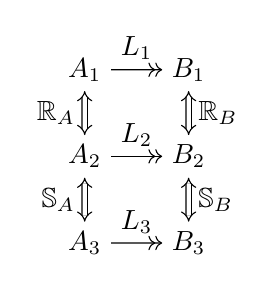
\begin{tikzpicture}[baseline=0.6mm,xscale=0.66,yscale=0.55]
    \node (A1) at (-1,  2) {$A_1$};
    \node (A2) at (-1,  0) {$A_2$};
    \node (A3) at (-1, -2) {$A_3$};
    \node (B1) at ( 1,  2) {$B_1$};
    \node (B2) at ( 1,  0) {$B_2$};
    \node (B3) at ( 1, -2) {$B_3$};
    \draw (A1) edge[->>] node[auto] {$L_1$} (B1);
    \draw (A2) edge[->>] node[auto] {$L_2$} (B2);
    \draw (A3) edge[->>] node[auto] {$L_3$} (B3);
    \begin{scope}[double equal sign distance, {Implies[]}-{Implies[]}]
      \draw (A1) edge[double] node[auto,swap] {$\mathbb{R}_A$} (A2);
      \draw (B1) edge[double] node[auto] {$\mathbb{R}_B$} (B2);
      \draw (A2) edge[double] node[auto,swap] {$\mathbb{S}_A$} (A3);
      \draw (B2) edge[double] node[auto] {$\mathbb{S}_B$} (B3);
    \end{scope}
  \end{tikzpicture}
  $
  \caption{Simulation identity and vertical composition}
  \label{fig:simcomp}
\end{figure}
%}}}

%}}}

%}}}
        % 3-4 pages
\section{Verified Compilation with a Nominal Memory Model}
\label{sec:nominal}

In this section, we describe the limitations of the block-based
memory model and present our new 
{\em nominal memory model} which removes the global constraints for
managing memory blocks and enables flexible memory structures for open
programs and concurrent threads.

\subsection{Problems with the Block-Based Memory Model}
\label{ssec:nominal-bbmm}

In the block-based memory model, the memory space is represented as a
countably infinite set of blocks where each block is given a unique
identifier called its \emph{block id} (denoted by $b$, represented
as postitive numbers). The entire memory space is
divided into two parts by a special block id called
\emph{\nextblock}. A block with id less than \nextblock has been
allocated (called a \emph{valid block}). Otherwise, it has not been
allocated yet (called an \emph{invalid block}). \nextblock---initially
with the value $1$---denotes the id of the next block to be allocated
and will be increased after each allocation. A valid memory block is a
finite array of bytes with a lower and upper bound. A \emph{memory
state} (denoted by $m$) consists of a mapping from addresses to
\emph{in-memory values} in valid blocks and the value of
\nextblock. Its type \coqe{mem} is defined in~\figref{sfig:memstate}
where \coqe{block} is the type of block ids, \coqe{Z} is the type of
integers, \coqe{memval} is the type of in-memory values, and
\coqe{$m$.(mem_contents) $b$ $o$ = $v$} iff $b$ is a valid block in
$m$ and $v$ is the in-memory value at the $o$-th memory cell (byte) of
$b$.

A pointer or a memory address is a pair $(b, o)$ where $b$ is the
memory block it points to and $o$ is an index to a memory cell in block
$b$ (also called an offset).
%
Pointer arithmetic is represented by adjustments to offsets. For
example, $(b, o) + n$ is defined as $(b, o+n)$.
%
This simple block-based abstraction already provides basic support for
memory isolation, in the sense that given a pointer to block $b_1$ we
can never reach $b_2$ by performing pointer arithmetic if $b_1 \neq b_2$.

\begin{figure}
  \begin{subfigure}[b]{.45\textwidth}
    \begin{coq}
Definition block : Type := positive.
Record mem: Type := { 
  mem_contents: block -> Z -> memval;
  nextblock: block; }.
    \end{coq}
    \caption{Blocks and Memory States}
    \label{sfig:memstate}
  \end{subfigure}
  \begin{subfigure}[b]{.5\textwidth}  
    \begin{coq}
alloc : mem -> Z -> Z -> mem \times block
free  : mem -> block -> Z -> Z -> $\some{\code{mem}}$
load  : mem -> chunk -> block -> Z -> $\some{\code{val}}$
store : mem -> chunk -> block -> Z -> val -> $\some{\code{mem}}$
    \end{coq}
    \caption{Memory Operations}
    \label{sfig:memops}
  \end{subfigure}
  \caption{Definitions for the Block-Based Memory Model}
  \label{fig:bbmem}
%  \vspace{-0.1cm}
\end{figure}

\figref{sfig:memops} shows the main operations over memory where
\coqe{val} is the type of \emph{regular values}:
%
\begin{coq}
   Inductive val := Vundef | Vint $i_{32}$ | Vlong $i_{64}$ | Vsingle $f_{32}$ | Vfloat $f_{64}$ | Vptr $(b,o)$.
\end{coq}
%
Here, \coqe{Vundef} represents undefined values, \coqe{Vptr $(b,o)$}
represents a pointer $(b,o)$, and the remaining forms denote 32- and
64-bit integer and floating point values.
%
\coqe{chunk} is the type of \emph{memory chunks} containing
information necessary for performing conversion between in-memory
values and regular values.
%
Note that the option type $\lfloor \rfloor$ is used to describe the
possible failure of some operations.  Given a memory state $m$, a
lower bound $l$ and a higher bound $h$, \coqe{alloc $m$ $l$ $h$}
returns a new block whose id is \coqe{$m$.(nextblock)} and whose valid
offsets are in the range of $[l,h)$. It also returns a new memory state
  where \nextblock is increased by $1$ and the newly allocated memory
  cells are initialized with undefined values.
%
Note that \coqe{alloc} \emph{always succeeds} because the memory space
has infinitely many blocks. The \coqe{free} operation frees memory
cells in a certain range. Given $m$, $k$ $b$ and $o$,
\coqe{load $m$ $k$ $b$ $o$}
loads a value starting from the address $(b,o)$ such
that the size and type of value are determined by $k$.  Conversely,
\coqe{store} stores a value into a certain location in memory.

A main task of compilers is to transform abstract data structures
(e.g., stacks) for describing the semantics of the high-level source
languages into concrete data structures for the low-level target
languages. These transformations often operate on certain part of
memory and have local effects.

CompCert introduces \emph{injections} to capture such changes. An
injection $j$ is a partial function of type
\coqe{block -> $\some{\code{block} \times \code{Z}}$}, such that $j(b) =
\some{(b',o)}$ iff a block $b$ is inserted into block $b'$ at offset
$o$ by the transformation. If $j(b) = \none$ (we use $\none$ to
represent the \coqe{None} constructor), then $b$ is removed from the
memory after the transformation.

When proving the correctness of these memory-transforming passes, one
would expect that we could exploit the locality of memory
transformations to construct intuitive proofs. For example, for
\code{SimplLocals}, \coqe{Cminorgen} and \coqe{Stacking}, one would
like to exploit the facts that \emph{1)} blocks for global definitions
are unchanged, and \emph{2)} the changes to individual stack frames
cannot interfere with each other. However, it is impossible to
formalize these facts directly because we can neither distinguish
blocks for global definitions from blocks in stack frames, nor tell
the differences between blocks in different stack frames: they are all
indexed by positive numbers. This problem is exactly caused by
\textbf{Inflexibility 1} introduced in~\S\ref{ssec:intro-nmm}.


Verification techniques for open programs are compositional only if
the semantics of open programs are compatible with each other.
However, the existence of a global \nextblock makes this compatibility
very difficult to establish, even when different open programs operate
on completely separate memory regions.
\ignore{
\begin{wrapfigure}[12]{r}{0.5\textwidth}
  \begin{tikzpicture}[scale=0.6, every node/.style={scale=0.9},auto]
    \def\bh{0.2cm}
    \tikzstyle{af}=[draw,minimum width=0.5cm, minimum height=0.5cm, rounded corners=.05cm];
    
    \node[af,fill=yellow] (t1f) {$f$};
    \node[af, below=\bh of t1f, fill=yellow] (t1g) {$g$};
    \node[af, below=\bh of t1g, pattern = north east lines] (t1i) {};
    \node[af, below=\bh of t1i, pattern = north east lines] (t1j) {};
    \node[af, below=\bh of t1j, fill=yellow] (t1h) {$h$};
    %% \node[draw = none, below left =\bh and -0.1cm of t1h, rotate = 90] (t1end) {$\ldots$};
    
    \draw[->,>=stealth] (t1f) -- (t1g);
    \draw[->,>=stealth] (t1g) -- (t1i);
    \draw[->,>=stealth] (t1i) -- (t1j);
    \draw[->,>=stealth] (t1j) -- (t1h);
    \draw[->,>=stealth] (t1h) -- ($(t1h.south) + (0cm, -0.3cm)$);

    \node[above = 0.1cm of t1f] {Thread $1$};

    \node[af, right = 2cm of t1f, pattern = north east lines] (t2f) {};
    \node[af, below=0.22cm of t2f, pattern=north east lines] (t2g) {};
    \node[af, below=\bh of t2g,fill=green] (t2i) {$i$};
    \node[af, below=\bh of t2i,fill=green] (t2j) {$j$};
    \node[af, below=\bh of t2j, pattern=north east lines] (t2h) {};
    %% \node[draw = none, below left =\bh and -0.1cm of t2h, rotate = 90] (t2end) {$\ldots$};

    \draw[->,>=stealth] (t2f) -- (t2g);
    \draw[->,>=stealth] (t2g) -- (t2i);
    \draw[->,>=stealth] (t2i) -- (t2j);
    \draw[->,>=stealth] (t2j) -- (t2h);
    \draw[->,>=stealth] (t2h) -- ($(t2h.south) + (0cm, -0.3cm)$);

    \node[above = 0.1cm of t2f] (t2txt) {Thread $2$};

    \node[draw=none, right = 1cm of t2i] (comp) {\large\bf $\Longrightarrow$};
    \node[draw=none, above = 0.1cm of comp] {\small \emph{Thread Linking}};

    \draw[->, dashed, >=stealth] (t1g) -- node [sloped, above] {\small \emph{yield}} (t2i);
    \draw[->, dashed, >=stealth] (t2j) -- node [sloped, above] {\small \emph{yield}} (t1j);


    \node[af, right = 3cm of t2f,fill=yellow] (tf) {$f$};
    \node[af, below=\bh of tf,fill=yellow] (tg) {$g$};
    \node[af, below=\bh of tg,fill=green] (ti) {$i$};
    \node[af, below=\bh of ti,fill=green] (tj) {$j$};
    \node[af, below=\bh of tj,fill=yellow] (th) {$h$};
    %% \node[draw = none, below left =\bh and -0.1cm of th, rotate = 90] (tend) {$\ldots$};

    \draw[->,>=stealth] (tf) -- (tg);
    \draw[->,>=stealth] (tg) -- (ti);
    \draw[->,>=stealth] (ti) -- (tj);
    \draw[->,>=stealth] (tj) -- (th);
    \draw[->,>=stealth] (th) -- ($(th.south) + (0cm, -\bh)$);
    
    \node[right = 2cm of t2txt] {Threads $\{1,2\}$};
    

  \end{tikzpicture}
  \vspace{-0.2cm}
  \caption{\scriptsize{}Linking of Multiple Stacks into a Single Stack in CCAL}
  \vspace{-0.2cm}
  \label{fig:stack-linking}
\end{wrapfigure}
}
We take the compilation and linking of Certified Concurrent
Abstraction Layers (CCAL) as an example to illustrate the above
problem~\cite{ccal18}.
\ignore{
A concurrent certified abstraction layer $L$
consists of shared and private memory states, abstract states, and a
set of possibly shared primitive operations (like external
functions). The semantics of a language (\eg, C or assembly) built on
top of $L$ forms an abstract machine in which concurrent programs can
be formally described.
}
%
A CCAL object is a formally verified open program built on top of some
layer $L$. A multi-threaded program is developed by abstracting
individual threads into CCAL objects. These objects are then
compiled by an extension of CompCert called Thread-Safe CompCertX into
assembly code. Finally, CCAL objects need to be linked together to
form a complete program. 

For the above linking to be possible, the views of memory of CCAL
objects must be compatible with each other. Achieving this
compatibility is non-trivial since 
a new stack block is
allocated for every function call in CompCert's assembly. To
link threads together, it is necessary for each thread to have
the same sequences of
stack blocks and \nextblock, meanwhile preventing one
thread from accessing the private stack memory of the others.
%
%
\ignore{
To solve the above problem, the authors of Thread-Safe
CompCertX~\cite{ccal18} modify the assembly semantics so that when a
thread yields to its context, a sequence of dummy stack blocks is
allocated to increase \nextblock in accordance with the actual
allocation of stack blocks by the context. Moreover, to avoid any
interference between memory operations on the stacks in different
threads, the dummy blocks do not carry any read or write
permission---they are ``dead'' memory cells from the perspective of
the focused thread. With those devices, it is possible to ``thread''
the private stack frames of each thread into a single stack. As an
example, the linking of stacks for two threads is depicted in
\figref{fig:stack-linking}. Here, the call to the yield primitive from
thread $1$ to $2$ in the function $g$ allocates two dummy blocks
(marked with diagonal lines) for the corresponding execution in thread
$2$. Accesses to these dummy blocks are invalid in thread $1$.


The solution above has two problems.
%
First, intuitively, each thread should have it own private stack:
the context should not interfere with operations on this stack.
Contrary to this assumption, the growth of dummy frames depends
on how contextual threads change \nextblock. This introduces
unnecessary complication to verification of compilation.
%
Second, in the linked program, stack frames for different threads are
interleaved with each other. This makes the semantics of
linked programs much more complex. It is also extremely difficult to
further verify their compilation to actual machine code where each
thread should have its own contiguous and private stack.
%
}
These problems are exactly caused by
\textbf{Inflexibilities 2 and 3} in~\S\ref{ssec:intro-nmm}.

\subsection{The Nominal Memory Model}
\label{ssec:nominal-nmm}

We solve the above problems by getting rid of the inflexibilites of
the block-based memory model through a generalization based on nominal
techniques.

Nominal techniques~\cite{pitts-nominal,gabby2002} provide a
mathematical foundation for managing named resources. 
%
In this setting, any countably infinite set $\nameset{A}$ can
represent a set of available names. Elements in these sets are called
\emph{atomic names} (or simply \emph{names} in short). Dependency of
objects upon names is captured by the notions of \emph{permutations}
and \emph{supports}. A permutation $\pi$ is a bijection from
$\nameset{A}$ to itself that only renames a finite subset of names in
$\nameset{A}$. Given a set of objects $X$ and some $x \in X$, $A
\subseteq \nameset{A}$ supports $x$ (or $A$ is a support of $x$) iff,
for any permutation $\pi$ on $\nameset{A}$ that is an identity mapping
for names in $A$, we have $\pi \cdot x = x$ where $\_ \cdot \_$
denotes the ``application'' (known as an \emph{action}) of $\pi$ to the
object $x$. This effectively means that $x$ is independent of any name
outside of $A$.
%
Only objects that can be supported by a finite set of names are of
interest to us.
%
A binary relation called \emph{freshness} makes the independence
relation concrete. A name $a\in \nameset{A}$ is fresh w.r.t. $x$
(written as $\freshness{a}{x}$) iff $x$ is supported by some finite set $A
\subseteq \nameset{A}$ and $a \not\in A$.

\begin{figure}[t]
\begin{coq}
  Module Type BLOCK.
    Parameter block : Type.
    Parameter eq_block : $\forall\app x\app y: \scode{block}, \sumbool{x=y}{x \neq y}$.
  End BLOCK.

  Module Type SUP.
    Parameter sup: Type.
    (** Operations *)
    Parameter sup_empty : sup.  (* Empty support *)
    Parameter fresh_block : sup -> block.  (* Generation of fresh blocks *)
    Parameter sup_incr : sup -> sup.  (* Increment of supports *)
    Parameter sup_in : block -> sup -> Prop.   (* Check validity of block ids *)
    (** Properties *)
    Parameter sup_dec : $\forall\app b\app s, \sumbool{\scode{sup\_in}\app b\app s}{\neg \scode{sup\_in}\app b\app s}$.
    Parameter empty_in: $\forall\app b, \neg \scode{sup\_in}\app b\app \scode{sup\_empty}$.
    Parameter freshness : $\forall\app s, \neg \scode{sup\_in}\app (\scode{fresh\_block}\app s)\app s$.
    Parameter sup_incr_in : $\forall\app a\app s, \scode{sup\_in}\app a\app (\scode{sup\_incr}\app s) 
    \leftrightarrow a = (\scode{fresh\_block}\app s) \lor \scode{sup\_in}\app a\app s$.
  End SUP.  
\end{coq}
  \vspace{-0.2cm}
  \caption{Interfaces of the Nominal Memory Model}
  \label{fig:nm-interface}
  \vspace{-0.1cm}
\end{figure}

The above concepts can be used to characterize the block-based
memory model. By taking memory states as objects containing names, 
we adopt the following analogies:
%
\begin{itemize}\itemsep 0pt
\item Block ids represent names that memory states depend upon;
\item Given a memory state $m$, the set of valid blocks in $m$
  represents a support of $m$;
\item Given a memory state $m$, its \nextblock is fresh w.r.t. $m$.
\end{itemize}
%
Note that the set of valid blocks is always finite. To some extent, the
existing memory operations in CompCert already exploit the properties
of atomic names and supports. For example,
\coqe{alloc} always succeeds because there is always an infinite amount
of ids outside the set of valid blocks.

However, the block-based memory also makes rigid assumptions
about names and supports:
%
\begin{itemize} \itemsep 0pt
\item Block ids are fixed to positive numbers;
\item For any memory state $m$ whose \nextblock is $n$, its support
  must be the fixed set of consecutive numbers $\{1,\ldots,n-1\}$;
\item For any memory state $m$ whose \nextblock is $n$, its fresh
  block must be assigned with the id $n$.
\end{itemize}
%

We remove these rigid assumptions and generalize the block-based
model into the nominal memory model by introducing an
abstraction of block ids and supports as module types, as shown
in~\figref{fig:nm-interface}.
%
By the definition of \coqe{BLOCK}, block ids are names with decidable equality.
%
By the definition of \coqe{SUP}, a support type must be accompanied by
four kinds
of operations: checking the membership of blocks in supports
(\coqe{sup_in}), creating an empty support (\coqe{sup_empty}),
generating fresh blocks (\coqe{fresh_block}) and increasing supports
with new blocks (\coqe{sup_incr}). Furthermore, those operations must
satisfy some well-formedness properties. 

\begin{figure}
\begin{coq}
  Module Block <: BLOCK.
    Definition block := positive.         Definition eq_block := peq.
  End Block.

  Module Sup <: SUP.
    Definition sup := list block.         Definition sup_in ($b$: block) ($s$: sup) : Prop := $b \in s$.
    Definition sup_empty : sup := [].     Definition fresh_block ($s$: sup) := (find_max_pos $s$) + 1.
    Definition sup_incr ($s$ :sup) := $(\scode{fresh\_block }s) \cons s$.   $\qquad$ ...
  End Sup.  
\end{coq}  
  \vspace{-0.2cm}
  \caption{Block-based Memory Model as an Instance}
  \vspace{-0.1cm}
  \label{fig:bm-instance}
\end{figure}

We also note that the above generalization does not exactly match with the
standard definitions in nominal techniques. For example, \coqe{BLOCK} does not
enforce that block ids are from a countably infinite set. Instead,
the \coqe{freshness} property guarantees that any block fresh w.r.t a
support $s$ must not be already in $s$. Together with the totality of
\coqe{fresh_block}, it implies the existence of an infinite number of
block ids.
%
We also define supports to be any type that has the interface of
\coqe{SUP}, instead of a finite set of block ids. This generalization
allows us to instantiate \coqe{sup} with complex data structures for
formalizing memory space in fine-grained styles. 

To make use of the above interfaces, we instantiate block ids and
supports as follows:
%
\begin{coq}
  Module Block <: BLOCK. ... End Block.           Module Sup <: SUP. ... End Sup.
\end{coq}
%
Then the original \coqe{block} type is instantiated with
\coqe{Block.block}. Moreover, the memory state carries a support instead of
\nextblock:
%
\begin{coq}
  Record mem: Type := { mem_contents: block -> Z -> memval;   support: Sup.sup;}.
\end{coq}
%
The memory operations are adapted accordingly. For example, checking
of valid blocks is done by using \coqe{sup_in} instead of comparing
with \nextblock:
%
\begin{coq}
  Definition valid_block ($m$:mem) ($b$:block) := $b$ < $m$.(nextblock).   (* Old *)
  Definition valid_block ($m$:mem) ($b$:block) := sup_in $b$ $m$.(support).  (* New *)
\end{coq}
%
For another example, \coqe{alloc} now invokes \coqe{fresh_block} to
allocate a new block instead of consulting \nextblock.
The properties of all memory operations can be easily reestablished
because they are already ignorant of particular instantiations of block ids
and supports. 

Finally, the block-based memory model becomes a special case of the
nominal memory model, as depicted in~\figref{fig:bm-instance} where
\coqe{find_max_pos} finds the maximal positive number in a list.

\vspace*{-2ex}
\paragraph*{Proposed Research.}
As a preliminary evidence for its effectiveness, we have recently
successfully applied the nominal memory model to the full compilation
chain of CompCert to get Nominal CompCert~\cite{wang2022}.  We updated
the semantics of every language of CompCert by replacing the old
memory operations with the new one. We then also updated the
simulation proofs. Because the generalization of block ids and
supports is mostly orthogonal to the simulation proofs in CompCert,
the changes are minimal.

\vspace*{-2ex}
\paragraph*{Task 2a: Nominal CompCert with structural memory space.}
A big part of our proposed effort is to develop various instantiations
of the nominal memory model where the whole {\em memory space} is
divided into memory regions with well-defined structures and clear
roles. One promising design~\cite{wang2022} separates global memory
(for global variables and functions) from stack memory; and then
organizes the stack into a tree structure that mirrors the ``call
activation'' tree.  Because most memory transformations do not change
the order of function calls and returns, the stack tree remains stable
under compilation; this allows us to recover the locality decompose a
transformation on the entire stack into local transformations on
individual stack frames, which could lead to much simpler and more
intuitive proofs for memory injection phases.

\vspace*{-2ex}
\paragraph*{Task 2b: Norminal CompCertO for open programs.}
Another key task is to integrate the norminal memory model into our
new compositional verified compilation framework in
\S\ref{sec:compcerto}.  Compositional compilation needs to not only
keep track of how memory is transformed by internal functions, but
also do that for external functions.  If the context is fixed, the
transformation on contextual memory should always be described as
\emph{an identity mapping} from source to target memory blocks,
regardless of how complicated the memory transformation is for
internal executions.  However, this seemingly simple task is extremely
difficult to complete in the original CompCert because it lacks the
ability to distinguish memory blocks allocated by internal functions
from those by external ones. With the nominal memory model and its
instances, contextual memory can be separated from internal memory and
be reasoned about via a well-defined interface, leading to simpler and
more elegant correctness proofs for compiling certain kinds of open
programs. We believe that these techniques together with others we
have built on top of the nominal memory model could be particularly
beneficial in the general context of compositional compiler
correctness.

\ignore{
In CompCert, the complexity of memory injections is largely confined
to the correctness proofs of individual passes: injections are
existentially quantified as part of the simulation relation and do not
appear in the correctness statement itself.  This is possible because
memory states are not part of the externally observable behavior of
programs. This assumption must be relaxed in compositional extensions
of CompCert which model interactions between compilation units.  In
work such as Compositional CompCert~\cite{compcompcert},
CompCertX~\cite{dscal15,wang2019}, CompCertM~\cite{compcertm},
CASCompCert~\cite{cascompcert} and CompCertO~\cite{koenig21}, memory
states appear as part of the interactions between components.  As a
consequence, the memory relations used by compilation passes become
part of their correctness statements.  This makes correctness theorems
and the vertical composition of passes much more complex.

Our techniques based on the nominal memory model have the potential to
significantly simplify the above proofs from the following
perspectives.  First, the evolving Kripke worlds used in compositional
compiler correctness are used to store both memory injections (which
can be determined ahead of time using more structural injection
functions) and additional permission information (which could be
stored in our model as part of the information associated with block
identifiers).  As a result, by incorporating our approach, it may be
possible to eliminate Kripke worlds entirely, which would
significantly simplify the semantic frameworks used in these projects.
Moreover, our techniques could help isolate private memory as internal
states, for example through the use of a partial commutative monoid
structure on memory states which would facilitate splitting and
merging private memory regions used by individual components.
Finally, they could provide a seamless way to incorporate stack
awareness to compositional compilers of this kind.
}

\vspace*{-2ex}
\paragraph*{Task 2c: Norminal CompCertO for open threads}
We will extend Nominal CompCertO to support
multi-threaded programs. The existing solutions invented ad hoc
mechanisms~\cite{ccal18} to cope with the global \nextblock which
prevent further compilation to a realistic machine model in which each
thread has its own contiguous and private stack. We plan to
instantiate supports with multiple stack trees where we can grow
the stacks individually without interference with each other, thereby
eliminating the problems with \nextblock.



          % 3-4 pages
\section{Compositional Verified Compilation into ELF Object Files}

Together with his students, PI Shao has recently developed
CompCertELF~\cite{compcertelf20}, the first extension to CompCert that
supports verified compilation from C programs all the way to a
standard binary file format, i.e., the ELF object format.  However,
CompCertELF only supports {\em{}verified separate
compilation}~\cite{sepcompcert} which cannot handle compositional linking of
heterogeneous components.  For this proposal, we will integrate the
technologies in CompCertELF into Nominal CompCertO to build an {\em
  end-to-end and compositional verified compiler} that can compile C
components all the way into ELF object files.

\vspace*{-2ex}
\paragraph*{Task 3a: Stack-Aware Nominal CompCertO.}
To support concrete memory layout required by the binary machine code,
we will first extend Nominal CompCertO to support compilation with a
single, continuous, and finite stack by incorporating the key ideas in
Stack-Aware CompCert~\cite{wang2019,compcertelf20}.  Stack-Aware
CompCert explicitly manages the call stack by adding a data type
called \emph{abstract stack} to memory states. The abstract stack
records the history of memory consumption incurred by stack allocation
and maintains fine-grained \emph{stack permissions}. By exploiting
that information, Stack-Aware CompCert achieves contextual compilation
of single-threaded C programs into an assembly language that is aware
of a single and finite stack.  In our structured nominal memory model,
the abstract stack can be readily absorbed into the support. We can
drop stack permissions from the abstract stack in Stack-Aware CompCert
because CompCertO already separately enforces them as part of its
reasoning framework (e.g., simulation conventions).  Furthermore, by
enriching supports with multiple abstract stacks following the idea of
Task 2d, we will build Multi-Stack Nominal CompCertO which can compile
multi-threaded programs onto multi-stack machine models. These ideas
will form a complete solution to thread-safe contextual compilation
needed to support CCAL~\cite{ccal18}.

\vspace*{-2ex}
\paragraph*{Task 3b: Verified compilation into relocatable ELF files}
CompCertELF is built on top of Stack-Aware CompCert. In essence, it
modifies and extends Stack-Aware CompCert's compilation chain with a
\emph{verified assembler} that transforms the realistic assembly
programs output by Stack-Aware CompCert to sequences of bytes that
represent relocatable ELF files.  This assembler consists of several
passes that successively merge code and data into atomic blocks (known
as sections), generate information for relocation and linking (such as
symbol tables and relocation tables), encode the assembly instructions
and the global data into their binary forms, and finally embed them
into the ELF format with meta-data (such as section headers and ELF
headers). A big part of this task is to leverage the rich structure
from the nominal memory model to enable richer ABIs.  Another
challenge is to develop automation support building certified
instruction encoders and decoders for different machine
architectures~\cite{xu21}.

\vspace*{-2ex}
\paragraph*{Task 3c: Certified compositional ELF linker and loader}
To support end-to-end certified linking, CompCertELF has to prove
compilation commutes with two different linkers: one used in CompCert
and the other for relocatable object files. On one hand, in CompCert,
the linker views programs as partial mappings from identifiers to
global definitions. Therefore, it is insensitive to and may
arbitrarily rearrange the order of definitions. On the other hand, to
generate relocatable object files, the function and variable
definitions are merged into atomic sections following some particular
order. The ELF linker simply concatenates sections of the same type
together like they are ``black boxes.''  Here, the order in which
definitions are merged and sections are concatenated significantly
affects the result of linking.  The consequence is that commutativity
between linking and compilation breaks at the transitional phase from
CompCert to the assembler where the latter links programs as
relocatable objects. We believe that the language interfaces in
CompCertO and the richer permutation support in our nominal memory
model can provide a better and cleaner solution toward a certified
linker and loader.

      % 1 page
%\documentclass[11pt]{article}
\usepackage{geometry}
\usepackage{amsmath}
\usepackage{amssymb}
\usepackage{hyperref}
\usepackage{libertine}
\usepackage[libertine]{newtxmath}
\usepackage{stmaryrd}
\usepackage{cmll}
\usepackage{bbm}

\title{Security properties in CompCertO/RBGS}
\author{J\'er\'emie Koenig}

\begin{document}

\maketitle

\begin{abstract} %{{{
In this document I summarize how I understand
secure compilation
in the context of CompCertO and refinement-based game semantics.
In a model with dual nondeterminism,
properties and hyperproperties
can be formulated as specifications.
Both are preserved by simple refinement as a result,
but the ways in which specific (hyper)properties interact with
a compiler's calling convention $\mathbb{C}$
must be investigated on a case-by-base basis.

For example, \emph{nonintereference} is
a special case of hyperproperty.
But since assembly-level contexts can potentially observe details
which are not visible at the C level,
noninterefence is not automatically preserved by CompCertO.
However,
source-level noninterference induces a target-level property
of noninterference \emph{up to $\mathbb{C}$}
which can be characterized precisely.

Based on this characterization,
I show how to equip the target program
with call wrappers which eliminate
the potential information leaks introduced by compilation
and turn noninterference up to $\mathbb{C}$
back into the full-blown version of target-level noninterference.
\end{abstract}
%}}}

\section{Specification model} %{{{

What follows is a tentative formalization of the model $\mathsf{NTree}$.
This model is similar in spirit to the one used in our LICS '20 paper
and it defines some kind of free monad in $\mathbf{CDLat}$,
but unlike in the LICS model,
non-deterministic choices do not commute with external operations.

\subsection{Interaction specifications} %{{{

A computation with external operations in an effect signature~$E$
can be specified with an \emph{interaction specification} of the form:
\begin{equation} \label{eqn:construct}
  x \in \mathcal{I}_E ::=
    \bigvee_{i \in I} \bigwedge_{j \in J}
      m_{ij} \big( x_{ijk} \big)_{k \in N_{ij}}
  \qquad \text{where} \quad
  (m_{ij} \mathbin: N_{ij}) \in E
\end{equation}
The notations $\bigvee, \bigwedge$ are respectively meant to denote
angelic and demonic choice
constituting the joins and meet of a refinement lattice.
As such it will be natural to omit unary choices from notations,
and likewise denote nullary choices with the corresponding
upper and lower bounds:
\begin{align*}
  m(x_k)_k &:= \bigvee_{i \in \mathbbm{1}} \bigwedge_{j \in \mathbbm{1}} m(x_k)_k
  &
  \bigvee_{i \in I} m_i(x_k)_k &:=
    \bigvee_{i \in I} \bigwedge_{j \in \mathbbm{1}} m_i(x_{ik})_k
    & \bot &:= \bigvee_{i \in \varnothing} ()
  \\ &&
  \bigwedge_{j \in J} m_j(x_k)_k &:=
    \bigvee_{i \in \mathbbm{1}} \bigwedge_{j \in J} m_j(x_{jk})_k
    & \top &:= \bigwedge_{i \in \varnothing} ()
\end{align*}

Note that we define interaction specifications inductively,
so on any ``branch'' within a term
the constructor (\ref{eqn:construct})
can only be applied a finite number of times.
However,
because the index sets $I$ and $J$ can be infinite,
we are able to model infinite computations
by ranging over finite approximations.

%We could also use the less ``algebraic'' and more ``computational'' notation
%$
%  \bigvee_{i \in I} \bigwedge_{j \in J} k \leftarrow m_{ij} \mathbin; x_k
%$
%and corresponding abbreviations.

%}}}

\subsection{Refinement lattice} %{{{

Interaction specifications are equipped with a form of refinement
such that
\[
  \bigvee_{i \in I} \bigwedge_{j \in J_i}
  m_{ij}\big(x_{ijk}\big)_{k \in N_{ij}}
  \quad\le\quad
  \bigvee_{u \in U} \bigwedge_{v \in V_u}
  q_{uv}\big(y_{uvk}\big)_{k \in R_{uv}}
\]
holds when
\[
  \forall i \, \exists u \,
  \forall v \, \exists j \mathbin.
  (m_{ij} = q_{uv}) \wedge
  \forall k \mathbin. (x_{ijk} \le y_{uvk})
  \,.
\]
We will consider the interaction specifications $x$ and $y$
to be equal when both $x \le y$ and $y \le x$.

This ordering induces a completely distributive refinement lattice,
where joins and meets can be computed as expected.
Consider a family of interaction specifications $(x_i)_{i \in I}$
which can each be written as
$x_i = \bigvee_{j \in J_i} \bigwedge_{k \in K_{ij}} m_{ijk}(y_{ijkl})_l$.
We can give the supremum and infimum as:
\[
  \bigvee_{i \in I} x_i \:=\:
    \bigvee_{(i, j) \in \sum_i J_i} \,
    \bigwedge_{k \in K_{ij}} \,
    m_{ijk}(y_{ijkl})_l
  \qquad \qquad
  \bigwedge_{i \in I} x_i \:=\:
    \bigvee_{u \in \prod_i J_i} \,
    \bigwedge_{(i, k) \in \sum_i K_{i u_i}}
    m_{i u_i k}(y_{i u_i kl})_l
\]

%}}}

\subsection{Sequential composition} %{{{

Interaction specifications can used to build an interaction specification monad.
For an effect signature $E$ and a set $V$ we define
\[
  \mathcal{I}_E(V) \: := \: \mathcal{I}_{E \oplus \{\eta v \mid v \in V \}}
  \,,
\]
which is the set of interaction specifications
over a version of the signature $E$ which has been extended
with a nullary operation $\eta v : \varnothing$
for each of the variables $v \in V$.
The action of $\mathcal{I}_E(-)$ on functions
transforms those terminal operations:
\begin{gather*}
  \mathcal{I}_E(f)\Big( \bigvee_i \bigwedge_j m_{ij}(x_{ijk})_k \Big) :=
    \bigvee_i \bigwedge_j \bar{f}\big(m_{ij}(x_{ijk})_k \big)
  \\
  \text{where}
  \quad
  \bar{f}\big(m(x_k)_k\big) =
  \begin{cases}
    \eta[f(v)] () & \text{if } m = \eta v () \\ 
    m(\mathcal{I}_E(f)(x_k))_k & \text{otherwise}
  \end{cases}
\end{gather*}
Then the monad's unit
$\eta : V \rightarrow \mathcal{I}_E(V)$ and multiplication
$\mu : \mathcal{I}_E(\mathcal{I}_E(V)) \rightarrow \mathcal{I}_E(V)$
are defined as
\begin{align*}
  & \eta(v) := \eta v () & \text{and} \quad &
  \mu \Big( \bigvee_i \bigwedge_j m_{ij}(x_{ijk})_k \Big) :=
    \bigvee_i \bigwedge_j \bar{\mu} \big( m_{ij}(x_{ijk})_k \big) 
 \\
  && \text{where} \quad & \bar{\mu}\big(m(x_k)_k\big) :=
  \begin{cases}
    x & \text{if } m = \eta x () \\
    m\big(\mu(x_k)\big)_k & \text{otherwise.}
  \end{cases}
\end{align*}

%}}}

\subsection{Strategy specifications} %{{{

We can give an interpretation of a signature $F$
by giving for each $(m \mathbin: N) \in F$
a~specification $\sigma_m \in \mathcal{I}_E(N)$
in another signature $E$.
We will say that
\[
  \sigma \in \prod_{(m \mathbin: N) \in F} \mathcal{I}_{E}(N)
\]
implements the signature $F$ in terms of the signature $E$,
and write $\sigma : E \rightarrow F$.

Combining $\sigma : E \rightarrow F$ with
a client specification $x \in \mathcal{I}_F$
yields a result $x\sigma \in \mathcal{I}_E$,
where every external operation occurring in $x$
is replaced with its implementation in $\sigma$.
Formally,
\[
  \Big( \bigvee_i \bigwedge_j m_{ij}\big(x_{ijk}\big)_k \Big) \sigma
  \::=\:
  \bigvee_i \bigwedge_j
    \big(k \mathbin\leftarrow \sigma_{m_{ij}} \mathbin; x_{ijk} \sigma \big)
  \,,
\]
where $v \mathbin\leftarrow x \mathbin; y$
denotes the Kleisli extension
$\mu \circ \mathcal{I}_E(v \mapsto y)$
being applied to $x$,
in this case instructing to continue the computation with $x_{ijk} \sigma$
if $\sigma_{m_j}$ yields the value $k$.

The operation described above serves as the basis for strategy composition.
Given the strategy specifications
$\sigma : E \rightarrow F$ and $\tau : F \rightarrow G$,
the composition $\tau \circ \sigma : E \rightarrow G$ is defined by
\[
  (\tau \circ \sigma)_m \: := \: \tau_m \sigma \: \in \: \mathcal{I}_E(N)
  \,,
  \qquad \text{where }
  (m \mathbin: N) \in G
  \,.
\]

%}}}

\subsection{Deterministic computations}

%}}}

\section{Security properties as specifications} %{{{

The specification model outlined in the previous section
departs from usual trace semantics approaches,
resembling free monad constructions like interaction trees more closely.
Nevertheless,
I will show below that
traditional trace properties and hyperproperties
can be reformulated as specifications within that model.

\subsection{Traces and properties} %{{{

As a system executes, we can record in a \emph{trace}
the observable interactions between the system and its environment
(and sometimes record the evolution of the system's internal state).
Trace semantics model a system's behavior as
the set of traces which may be observed as the system executes.

Under this traditional setup,
desirable aspects of system behavior
can be described as \emph{trace properties}.
A trace property is simply a predicate which identifies
acceptable traces.
A system satisfies a trace property when
every one of its traces is acceptable.


%}}}

\subsection{Safety properties} %{{{

\emph{safety} property:
\[
  \bigvee_{q_1} \bigwedge_{r_1 \mid q_1 r_1 \in P}
  \bigvee_{q_2} \bigwedge_{r_2 \mid q_1 r_1 q_2 r_2 \in P}
  \cdots
\]

\[
  \bigwedge_{i \in I} m_i \Big(
  \bigwedge_{j \in J_{iu}} m_{iuj} \Big(
  \bigwedge_{k \in K_{iujv}} m_{iujvk} \Big(
  \cdots
  \Big)_w
  \Big)_v
  \Big)_u
\]

\begin{align*}
  \phi P &:= \{ q \mid qrs \in P \}  \quad \text{(first action)} \\
  qr \backslash P &:= \{ s \mid qrs \in P \} \quad \text{(residual)}
\end{align*}

\[
  \Sigma : \mathbf{Prop} \rightarrow \mathbf{Spec}
  \qquad \qquad
  \Sigma := \mu F \mathbin. \bigvee_{q \in \phi[P]}
    \underline{q} \big( F(\rho_{qr}[P]) \big)_r
\]

%}}}

\subsection{Hyperproperties}

%}}}

\section{Data abstraction and noninterference}



\section{Secure compilation}

We have seen that properties and hyperproperties
are special cases of RBGS specifications.
As such they are preserved by simple refinement.
However,
the data abstraction component of a compiler's correctness property





\section*{Old model}

The specification model has:
\begin{itemize}
  \item finite traces of the form $q_1 r_1 q_2 r_2 \cdots q_n r_n$;
  \item a refinement ordering $\le$, with
  \item unbounded angelic choices $\bigvee_{i \in I} x_i$ and
  \item unbounded demonic choices $\bigwedge_{i \in I} x_i$.
\end{itemize}
The \emph{finite trace} $q_1 r_1 q_2 r_2 \cdots q_n r_n$
can be interpreted as an elementary specification requiring that:
\begin{quote}
  If the system is invoked with a question $q_1$,
  its response will be $r_1$;
  if it is then invoked with a new question $q_2$,
  its response will be $r_2$,
  and so on.
\end{quote}
The \emph{refinement} $\sigma \le \tau$
means that the specification $\tau$ is more strict than $\sigma$.
In other words $\tau$ imposes at least the same requirements as $\sigma$,
and any system which satisfies $\tau$ will satisfy $\sigma$ as well:
\begin{align*}
  \sigma \le \tau
  \:\:\Longleftrightarrow\:\:
  \mathrm{Requirements}(\sigma) &\subseteq
  \mathrm{Requirements}(\tau)
\end{align*}
From the definitions above we can see
the prefix ordering of traces is a special case of refinement:
\[
  q_1 r_1 \:\le\: q_1 r_1 q_2 r_2 \:\le\: \cdots \:\le\: q_1 r_1 q_2 r_2 \cdots q_n r_n
  \,,
\]
since longer traces impose additional requirements
compared with their prefixes.


\paragraph{Refinement lattice}

Specifications constitute a complete lattice under the refinement ordering.
\emph{Angelic} choices let the \emph{user} of the system
pick which specification they wish to rely on,
and \emph{demonic} choices let the \emph{implementer} pick.
They are the join and meet of the refinement lattice:
\[
  \bigvee_{i \in I} \sigma_i \:\le\: \tau
  \:\:\Leftrightarrow\:\:
  \forall i \in I \mathbin. \sigma_i \le \tau
  \qquad \qquad
  \sigma \:\le\: \bigwedge_{i \in I} \tau_i
  \:\:\Leftrightarrow\:\:
  \forall i \in I \mathbin. \sigma \le \tau_i
\]
Note that
an infinite trace $t$ can be represented as
a limit $\bigvee \mathsf{FP}(t)$ of its finite prefixes
$s \in \mathsf{FP}(t)$.

\paragraph{Implementations}

Usually,
the point of a specification $\sigma$ is to
eventually construct a system $x$ which satisfies it.
We use the same kind of mathematical objects
to represent specifications and implementations,
and will state the correctness of $x$ with respect to $\sigma$
as the refinement $\sigma \le x$.
However,
not every specification represents a possible implementation.

Compared with general specifications,
implementations exhibit a well-defined behavior
which can only be influenced by observable inputs.
In other words,
implementations take the form
$x = \bigvee S$
where $S$ is a set of pairwise coherent traces.
Traces are coherent when
the same inputs lead to the same outputs:
\[
  s \coh \epsilon \qquad\qquad
  \epsilon \coh t \qquad\qquad
  q_1 r_1 s \coh q_1' r_1' t
  \: :\Leftrightarrow \:
  (q_1 = q_1' \Rightarrow r_1 = r_1' \wedge s \coh t)
\]
I will write
\[
  \mathbf{Impl} := \Big\{ \bigvee S \mathrel\Big|
    \forall s, t \in S \mathbin. s \coh t  \, \Big\}
  \qquad \text{and} \qquad
  \mathrm{Impl}(\sigma) :=
    \{ x \in \mathbf{Impl} \mid \sigma \le x \}
  \,.
\]
We can observe that:
{\small \[
  \sigma \le \tau
  \:\:\Longrightarrow\:\:
  \mathrm{Impl}(\sigma) \supseteq
  \mathrm{Impl}(\tau)
\qquad
  \mathrm{Impl} \Big( \bigvee_{i \in I} \sigma_i \Big) \: = \:
  \bigcap_{i \in I} \, \mathrm{Impl}(\sigma_i)
\qquad
  \mathrm{Impl} \Big( \bigwedge_{i \in I} \sigma_i \Big) \: = \:
  \bigcup_{i \in I} \, \mathrm{Impl}(\sigma_i)
\]}%
However,
specifications are not completely characterized
by their set of implementations,
and even nonimplementable specifications
may be non-trivial.
For example, the specification
\[
  \sigma = q r \vee q' r_1 \vee q' r_2
  \qquad \text{where} \qquad
  r_1 \neq r_2
\]
is not implementable,
but it could appear as a component in a larger specification
$\tau \circ \sigma$ which is.
For example $\tau$ may not invoke the overconstrained $q'$ at all,
or could react in the same way to the answers $r_1$ and $r_2$.



\end{document}
       % 2 pages
\section{Evaluation and Integration}

Talk more about supporting CCAL, CertiKOS, and DeepSEA


\paragraph*{Task 5a: CompCertX-style linking of CCAL layers (c and assembly layers).}
blah blah blah.

\paragraph*{Task 5b: End-to-end security-preserving refinement for CertiKOS.}
blah blah blah.

\paragraph*{Task 5c: Develop the DeepSEA backend and VST backend for building end-to-end verified user-level application on certified OS kernels.}
blah blah blah.


PIs should include a plan to evaluate the approaches developed as part
of the Project Description. Appropriate methods will depend on the
research area, topic, size and scope of the proposed project. Examples
include, but are not limited to, peer review of developed theories and
proofs, controlled experiments on appropriate
simulators/emulators/testbeds, user studies, or prototype
deployments. The plan should be appropriate for the size and scope of
the project.
       % 1 page
\section{Schedule and Milestones}

A detailed schedule of milestones are described as follows.
We will work on Tasks 1a, 1b, 1c throughout the duration of the project,
making necessary adjustments as we progress on other tasks
which depend on them.
In Year 1, 
we will complete Tasks 2a and 2b to
create an initial version of Nominal CompCertO for open programs,
and complete the parts of task 4a concerning sequential code only.
In Year 2, we will complete Tasks 2c, 3a, 4a, and
develop a prototype version of 3b and 4b.
In Year 3, 
we will complete Tasks 3b, 4b, 3c,
and start working on 4c.
In Year 4, we will complete Tasks 4c, 4d and 4e.

%[TODO: add mitigation plan of some kind,
%maybe dependency graph to show concurrent work?]

         % 0.5 pages
\section{Broader Impacts}
\label{sec:impact}

\paragraph*{Technology Transfer}
The proposed project aims at developing a compositional verified
compiler toolchain for C and related languages and creating a {\em
  certified} application binary interfaces (ABIs) for future
trustworthy heterogeneous systems. Such certified toolchain and ABIs
will greatly facilitate the verification of large-scale system
software, which in turn have a profound impact on the software
industry and the society in general.
Artifacts resulting from the project will be
made open-source to ensure rapid dissemination of ideas.

We plan to aggressively pursue technology transfer through several
different channels. First, PI Shao is the co-founder of CertiK,
a startup focusing on formal verification and auditing of smart
contracts and blockchain ecosystems. To date,
CertiK has provided services to over 1,800 clients and detected
over 31,000 vulnerabilities in blockchain code. It has also
successfully raised \$150 million of VC funding. CertiK has retargeted
DeepSEA to build verified smart contracts and developed a new
verified compiler backend for generating EVM code. We believe
that our new compositional verified secure compilation technology
can be readily applied to greatly enhance the power of this version
of DeepSEA as well.

Second, together with his Columbia colleagues, PI Shao is working on
a DARPA V-SPELLS project (called REFUEL)
which aims to develop verified composition and flattening of secure
enclaves for cyber-physical systems with large legacy code base.
REFUEL will deploy SeKVM and CertiKOS on the self-driving car
and UAV platforms to build VM-based and ARM-TrustZone-based secure
enclaves. The compositional compilation and verification technologies
developed in this proposal will be tested and transferred into realistic
case studies under the DARPA project.

\vspace*{-2ex}
\paragraph*{Curriculum Development}
We plan to develop innovative certified system software and formal
verification curriculum at both the undergraduate and graduate
level. The two PIs plan to develop a new course on Formal Semantics
(CPSC 430) at Yale based on the Nominal CompCertO developed in this
project. Existing courses and textbooks on formal semantics focus on
somewhat outdated material and do not cover exciting new technologies
such as game semantics, nominal techniques, and verified
compilation. By using our verified compiler toolchain as the basis, we
plan to create a set of programming labs where students can learn
modern compositional techniques through a more hands-on approach.

PI Shao also plans to revamp his course on Language-Based Security
(CPSC 428) based on the verified OS kernel (CertiKOS) and hypervisor
(SeKVM) and compiler toolchain (Nominal CompCertO) and certified
programming tools (DeepSEA and VST) where students can gain hands-on
experience on both system design and verification. We plan to extend
the courses to undergraduate and Master's research program where
students can participate in the proposed research. We will make our
course materials freely available and encourage our colleagues to use
them at other universities.

\vspace*{-2ex}
\paragraph*{BPC Plan and Outreach}
The supplemental BPC document contain a detailed plan on how the PIs
will engage in the wide range of BPC activities organized by the
Computer Science department at Yale. In addition, the PIs will
continue to recruit women and people from URGs (Under Represented
groups) to research.  PI Shao has a strong track record of mentoring
women and URGs in the past few years: he is currently serving as the
PostDoc advisor and mentor for the 2021 Computing Innovation (CI)
Fellow Anitha Gollamudi; he was the PostDoc advisor for Dr. Jung-Eun
Kim during 2017-2021, an MIT EECS Rising Star and now Assistant
Professor of Computer Science at NCSU; he was also the research
advisor for Valerie Chen during 2018-2020, a CRA Undergraduate
Research Award Finalist and now a PhD student at CMU.  If this project
is funded, the PIs will seek undergraduate students – especially women
and underrepresented minorities – through programs like REU to join
the work on building end-to-end verified compilation toolchain.


           % 1 page

\section{Results from Prior NSF Support}
\label{ssec:prior}

\paragraph{Expedition in Computing: The Science of Deep Specification (PI: Zhong Shao)} 
NSF CCF-1521531, \$2,046,445, with Andrew Appel and Lennart Beringer
(Princeton), Benjamin Pierce and Stephanie Weirich and Steven
Zdancewic (U. Pennsylvania), and Adam Chlipala (MIT), 2015-2020.  {\em
  Intellectual Merit:} The Yale Component of this expedition project
aims to develop a concurrent certified OS kernel (CertiKOS) and
connect it with the verified RISC-V hardware (developed at MIT) and
the web server (developed at UPenn, and verified at Princeton). The
key emphasis is to work out the detailed specification for the machine
interfaces (e.g., for RISC-V) and the system call interface (e.g., for
CertiKOS) so that software and hardware components verified by
multiple DeepSpec groups can indeed be linked togher. During the first
two years, The Yale team has successfully developed a clean-slate
CertiKOS hypervisor OS kernel that runs successfully on both Intel and
AMD multicore platforms with hardware virtualization and can boot
Ubuntu or Debian Linux as guest~\cite{certikos16}.  We have also
developed a new compositional approach for formally specifying and
verifying sequential and concurrent OS
kernels~\cite{chen16,costanzo16,certikos16}.  {\em Broader Impacts:}
This award has partly supported multiple postdocs and students in the
past two years. PhD student Ronghui Gu will join Columbia CS as a new
tenure track Assistant Professor.  The team has organized multiple
outreach workshops in 2016-2017, and also a two-week DeepSpec summer
school in 2017 with more than 150 attendees from all over the
world. PI Shao has incorporated the layered CertiKOS kernel into an
innovative undergraduate OS class.  {\em Representative Publications}:
two PLDI papers~\cite{chen16,costanzo16} and one OSDI
paper~\cite{certikos16}.

\paragraph{Co-PI Jeremie Koenig}
There is no prior NSF support for which Koenig is a PI.

            % 0.5 pages

\newpage
%%%%%%%%%%%%%%%%%%%%%%%%%%%%%%%%%%%%%%%%%%%%%%%%%%%%%%%%%%%%%%%%%%%%%%%%%%%%
%\section{References Cited}
{\bibliographystyle{abbrv}
\makeatletter
\renewcommand\small{%
   \@setfontsize\small{10.46}{12.77}
   \abovedisplayskip 10\p@ \@plus2\p@ \@minus5\p@
   \abovedisplayshortskip \z@ \@plus3\p@
   \belowdisplayshortskip 6\p@ \@plus3\p@ \@minus3\p@
   \def\@listi{\leftmargin\leftmargini
               \topsep 6\p@ \@plus2\p@ \@minus2\p@
               \parsep 3\p@ \@plus2\p@ \@minus\p@
               \itemsep \parsep}%
   \belowdisplayskip \abovedisplayskip
}
\makeatother
 \small\bibliography{references,shao,wang}
} \newpage
%%%%%%%%%%%%%%%%%%%%%%%%%%%%%%%%%%%%%%%%%%%%%%%%%%%%%%%%%%%%%%%%%%%%%%%%%%%%

\end{document}

